% <preamble>
\documentclass[12pt,a4paper,dvips]{article}
\usepackage{graphicx,xspace,overcite,amsmath}

\usepackage[dvips,
	bookmarks,
	colorlinks=true,
	hyperindex=true,
	hyperfigures,
	bookmarksnumbered=true]{hyperref}

\def\mydash{${-}$}
\newcommand{\D}{\displaystyle}
\newcommand{\etal}{{\it et al.}}
\sloppy

% </preamble>
% <document>
% <frontpage>
\begin{document}
\title{GMIN User Guide}
\author{David J.~Wales}
\date{Last updated \today}
\maketitle

\clearpage
\phantomsection
\pdfbookmark[0]{\contentsname}{contents} % Sets a PDF bookmark for the Table of Contents
\tableofcontents
% </frontpage>
% <intro>
\section{Introduction}

GMIN is a program that attempts to find the global potential energy minimum
for a collection of atoms or molecules using the `basin-hopping' algorithm
described by Wales and Doye.\cite{walesd97a}
A constant temperature Monte Carlo (MC) run is performed on the transformed
potential energy surface (PES), and the configuration point may either be reset 
to the latest minimum in the chain or vary freely.
The program knows many different empirical potentials, and it is straightforward to add new systems.
From version 2.2 basin-sampling thermodynamics has been added, and from 
version 2.3 parallel tempering basin-sampling and basin-hopping have been
implemented with MPI.

To start a calculation you need a file called {\tt data} in the current directory,
along with a file called {\tt coords} containing the initial coordinates,
which can be random. If the {\it SEED} keyword is present in
{\tt data} you also need a file called {\tt seed} containing the seed coordinates.
Most output is written to stdout, although the file {\tt lowest} is always created
at the end of the run, containing the energies and geometries of the lowest few
configurations found in the given run. The geometries are saved in XMakemol xyz format.

\section{New Options in GMIN.2.x}

From version 2 onwards GMIN was recoded in fortran90. 
Dynamic memory allocation is now used, so there are no hard limits on parameters
such as the number of atoms.
A number of new keywords have also been added since the first version of the code,
as well as numerous potentials.
The most important are probably {\it SYMMETRY}, {\it AVOID}, and {\it COOPMOVE}, which 
are directly used in global optimisation, 
and {\it HISTOGRAM}, which specifies a `basin-sampling' calculation of the energy
density of states.
A new algorithm (bipartite matching) has also been introduced for use with {\it PERMDIST}
and {\it AVOID} to deal with permutational isomers.
The implementation of {\it PERMDIST} is now the same as in OPTIM
and PATHSAMPLE, with a {\tt perm.allow} file to specify groups of permutable
atoms and secondary sets that can only permute together.
Finally, GMIN has been interfaced with CHARMM in much the same way as OPTIM, and there
are new keywords to specify how the current geometry should be perturbed in the
step-taking process. Keyword {\it CHARMMTYPE} specifies the type of CHARMM potential,
while {\it CHPMAX}, {\it CHPMIN}, {\it CHNMAX}, {\it CHNMIN},
{\it NOPHIPSI}, and {\it TOMEGA} govern the step-taking procedure in {\bf charmmgmin.src}.
Keyword {\it INTMIN} specifies that minimisation should be performed in internal coordinates,
but this seems to be slower than Cartesian coordinates in general.

Also new from version 2.3, the global minimisation basin-hopping algorithm has been enhanced with a 
parallel tempering option, which is implemented using MPI. Please see the notes
in the Makefile when loading compilers and MPI libraries. 
(Note that the LAM MPI 32-bit library is currently broken! MPICH has not been tested yet.)
The keyword {\it MPI} specifies
the number of processors for the parallel job and {\it BHPT} allows the user to specify the temperature
range over which the replicas are exponentially distributed and the probability of attempting 
an exchange.

Currently under development is a new implementation of basin-sampling where 
the quench probability for local minima is obtained using parallel-tempering rather than
a flat-histogram Wang-Landau method. This approach also employs MPI and can be invoked with 
the keyword {\it BSPT}.

\subsection{Basin-Sampling using {\it HISTOGRAM} and {\it TETHER}}

The `basin-sampling' algorithm as described by Bogdan, Wales and Calvo \cite{BogdanWC06} 
combines the `basin-hopping' \cite{walesd97a} and Wang-Landau 
sampling techniques \cite{wangl01} to study the thermodynamics of the transformed PES.
It provides a direct temperature-independent estimate of the total energy density of states,
along with thermodynamic properties such as the free energy and entropy via ensemble averages using
samples of local minima, rather than instantaneous configurations.

In the GMIN implementation setting {\it TEMPERATURE}
to zero and specifying the keyword {\it HISTOGRAM} invoke a `basin-sampling' run. 

In the microcanonical `basin-sampling' 
procedure we start from a random configuration and perform a random walk in energy space
by perturbing and minimising the structures. Assuming that a given energy is visited with probability
reciprocal to the true density of states, 
we obtain a flat energy distribution. To restrict the search of configuration
space to  bound clusters, the structures are confined to a spherical container. 
For every visited state the current estimate of the energy density of local minima
is updated by a multiplicative modification factor $f$ ({\it histfac}). 
Acting as a convergence parameter, $f$ is relatively large at first to allow for
fast accumulation of the histograms over the full energy range, 
and over time it is self-consistently reduced towards unity.
The length of one WL iteration, over which the value of the
modification factor stays the same, is regulated by the 
`flatness parameter' $x \%$ ({\it hpercent})---the percentage by which histogram entries
are allowed to deviate from the mean. As $f$ approaches a predefined 
value $f_{final}$ ({\it histfacmin}), and provided the random walk is unbiased
and all the energy levels are sampled uniformly, the energy density of local
minima converges to its true value. If 
the {\it VISITPROP} keyword is specified, the convergence of one WL iteration is governed by
the number of visits being proportional to $1/\sqrt(\ln(f))$\cite{ZhouB03}.

The energy spectrum in question is bounded from below by the potential energy of the global 
minimum {\it histmin} and is separated into {\it hbins}  
equally spaced energy windows, which constitute histogram bins of width {\it histint}. 

For a random configuration the probability of quenching to a minimum with potential energy 
lying in a given bin {\it i}  is
$g_i=p_i A_i$, where $p_i$ is the probability of a random minimum having potential
energy in a given bin, and $A_i$ is the average configuration space volume
of a basin of attraction for minima in this range. In the original
basin-sampling study $A_i$ is approximated by 
$\langle D_i \rangle ^{\kappa} $, 
where $\langle D_i \rangle$ is  the mean distance of a random starting point to the quenched minimum in the
corresponding bin, and  $\kappa$ is the number of vibrational degrees of freedom. 

During the random walk we accumulate
$g_i$ (the density of local minima in each bin---{\it hweight}), 
$H_j$ and $\overline{H}_j$ (the global energy histogram {\it histvals} and the
local energy histogram {\it lhistvals}, i.e.~the
number of visits in a given energy bin during one WL iteration), 
and $\langle D_j\rangle$ ({\it hdist}), which is updated when a new quenched minimum is added
to the corresponding bin. 

The run is started from a uniform energy distribution, $g_i$, 
and samples the configuration space with a probability inversely
proportional to $g_i$.
At each step all the Cartesian coordinates are displaced by a random number in the
range $[-1,1]$ times STEP.
The structure obtained after each geometrical perturbation is then minimised
using the modified limited memory Broyden-Fletcher-Goldfarb-Shanno (L-BFGS) algorithm\cite{lbfgs}. 
In the case of an atom leaving the container at any point the coordinates are 
reset to the starting geometry, and the previous minimum is recounted.  If the
minimisation is successful, the weights of the bins to which the starting ($i$) 
and the quenched ($i^\prime$) minima belong are compared . If
$g_i > g_{i'}$, the density of states of the
$i^\prime$-th bin is updated as $g_{i'} \rightarrow g_{i'} f$,
its energy histograms are incremented as  
$H_{i'} \rightarrow H_{i'} +1$ and $\overline{H}_{i'} \rightarrow \overline{H}_{i'} +1$, and the distance
between the starting and the quenched geometries is used to update $\langle D_{i'}\rangle$.
If $g_i < g_{i'}$  the attributes of the  $i$-th bin are modified instead. 
If the walk goes outside the defined energy range
we recount the structure in the $i$-th bin to avoid boundary effects.  After updating the histogram
we do not reset the coordinates at each successful step to those of the quenched minimum 
but allow the geometry to vary
continuously. The opposite strategy is generally found to be more effective for global optimisation, 
but here we must maintain detailed balance.

The energy histograms are periodically checked against the convergence criterion . 
Because the energy spectrum is discrete some energy bins may never be visited.  
Also, to prevent trapping when $f$ is close to
$f_{final}$,  bins where $H_i$ has fewer than $5 \%$ of the average number of entries are 
ignored by setting the {\it ignorebin} flag
to true. When the non-zero parts of the
histogram are considered sufficiently flat,
the modification factor is reduced using
a square root function, the values of $\overline{H}$ are reset and another WL iteration is started. 
The final statistical weights, $g_i$, can be used to calculate the canonical partition function in 
terms of contributions from the catchment basins in each energy range $i$.  

The geometries of minima can be saved along the run by specifying {\it BINSTRUCTURES } keyword. Keyword {\it EQUILIBRATION}
regulates the starting point and frequency of recording statistics.

The output of the `basin-sampling' run is printed in {\tt BL.Pjnorm.lnGj.Djnm.Djm.VT.his} in the
following format: 
{\it histmin}+(i-1/2)$\cdot${\it histint}; {\it hweight}(i)$\cdot$({\it distmin}/{\it dist(i)})$^\kappa$ 
normalised to $1$; ${\it \ln(hweight}(i))$ normalized to $1$;
average {\it hdist}(i) minimised with respect to rigid body coordinates; unminimised average 
{\it hdist}(i); {\it histvals}(i). 

Calculation of the
vibrational density of states for a given minimum is invoked by 
the additional {\it TETHER} keyword, which
requests a conventional Wang-Landau sampling of the configuration 
space restricted to the average volume of the basin of
attraction to which a given minimum belongs.\cite{BogdanWC06}

\section{The {\tt data} file}

Input is keyword driven with sensible defaults in most cases. 
Free format may be used within each line. Blank lines are ignored.

The following keywords are recognised, where {\it n\/} and {\it x\/} are integer and
real data, respectively.
\smallskip
% </intro>
\begin{itemize}
% <kwd>
\item {\it 2D\/}: enforce two-dimensional `flatland'.

\item {\it A9INTE\/}: specifies that after each quench that does not lead to an inversion of chirality, 
isomerisation of a peptide bond or cold fusion - the interaction enthalpy between a specified residue and the rest of the system
should be calculated using the external script `AMBGMINintE.sh', and read back into GMIN. This is intended for
use with protein/ligand systems where you are searching for low energy docked structures. As the total energy
does not fully correlate with the protein/ligand interaction enthalpy, it is often useful to retain not only the
lowest {\it SAVE\/} total energy structures, but also the lowest {\it SAVEINTE\/} interaction enthalpy structures.
To use this keyword, the `AMBGMINintE.sh' script (contained in the SVN repository in the SCRIPTS directory) must
be present in the GMIN working directory. You should ensure that you have edited it to match the residue numbering
of your system. You also need a full AMBER9+ installation with access to the `sander' executable. When using this
keyword, an interaction enthalpy dump file is produced every {\it DUMPINT\/} steps, and at the end of the run, 
structural output files are produced for the {\it SAVEINTE\/} lowest interaction enthalpy geometries. After each quench, 
the structure with the current lowest interaction energy is dumped in pdb and rst format prefixed with `bestint.' to allow
monitoring.

\item {\it ACCEPTRATIO accrat\/}: {\it accrat\/} is the required acceptance ratio for the MC
exploration of the transformed surface. For fixed temperature runs (the default) the maximum step size
is adjusted to try and meet the requested value of {\it accrat\/}; for a fixed maximum
step size the temperature is adjusted instead. The default value of {\it accrat\/} is a half.

\item {\it Ackland id\/}: specifies an Ackland embedded atom metal potential% \cite{} 
coded by Dr Mihai-Cosmin Marinica.
{\it id} specifies the particular metal: 1 is ?, 2 is ?, 3 is ?, 4 is ?, 5 is iron, 6 is a different iron,
7 is tunsten.
Positive values for {\it id} specify periodic boundary conditions, where box lengths must be
specified by the {\it PERIODIC\/} keyword. 
Negative values for {\it id\/} specify a cluster calculation. A {\it CUTOFF\/} value can also
be used for clusters.

\item {\it ALGLUE\/}: specifies a glue potential for aluminium.

\item {\it AMBER9 inpcrd inpcrdformat\/}: specifies a calculation with the interfaced
version of the Amber 9 program package. From this package the Amber force fields
are being used, with small modifications ({\it e.g.} smooth cut-offs).
Starting coordinates do not need to be specified in the {\it odata} file, they
are read from {\it inpcrd} instead (default {\it coords.inpcrd}), in Amber inpcrd
file format specified by the second optional argument {\it inpcrdformat}.
If the second argument is missing, it is assumed that {\it inpcrd} contains
only three columns with the xyz coordinates of all atoms, in the same order
as in the topology file. To start a run with this interface,
several auxiliary files are required in the same directory: input coordinate file
{\it coords.inpcrd}, parameter topology file {\it coords.prmtop},
input file to Amber containing force field specifications {\it min.in}, and, if
desired, a coordinate file different from {\it coords.inpcrd} containing
starting coordinates.
To turn on smooth cutoffs for the Generalised Born force fields, the keyword
{\it ifswitch=1} has to be used in the {\it \&cntrl} namelist block of {\it min.in}.
When using the {\it AMBER9} keyword, any calculated second derivatives will be
numerical. If one wants analytical second derivatives, the {\it NAB} keyword
should be used instead, with the same syntax. 
Additional keywords for the AMBER 9 runs are {\it DUMPSTRUCTURES}, {\it AMBERMDSTEPS},
{\it LIGMOVE (0.0-1.0) (x.x)} and {\it MOVABLEATOMS}.
% missing AMH - put it in after merger

\item {\it AMCHNMAX\/}: The maximum number of angles that will be changed by up to {\it STEP\/} during an 
AMBER dihedral step. If this is not set or is set to zero, cartesian steps of maximum size {\it STEP\/} are taken 
instead. 

\item {\it AMCHNMIN\/}: The minimum number of angles that will be changed during an AMBER dihedral step.

\item {\it AMCHPMAX\/}: The maximum probability for a single angle to be twisted in an AMBER dihedral step.

\item {\it AMCHPMIN\/}: The minimum probability for a single angle to be twisted in an AMBER dihedral step.

\item {\it ANGSTROM\/}: specifies coordinates in \AA ngstrom for the {\it FRAUSI\/}
potential.

\item {\it ARGON\/}: introduces a diatomics-in-molecules calculation for
a neutral, cationic or electronically excited argon cluster. See also
{\it GROUND\/}, {\it PLUS\/}, {\it TWOPLUS\/} and {\it STAR\/}.

\item{\it ARM arma armb}: use the acceptance-ratio method (Bouzida et al., {\it Phys.~Rev.~A},
{\bf 45}, 8894, 1992)  to adjust the step size to achieve the requested 
acceptance ratio. A scaling factor is calculated and applied to {\it step}, {\it rotmax},
and/or {\it transmax}. The scaling factor is calculated according to 
$\log(arma*P_{\rm t}+armb)/\log(arma*P_0+armb)$, where $P_{\rm t}$ defines the
target acceptance ratio and $P_0$ the actual acceptance ratio. Both values {\it arma} and
{\it armb} default to 0.4.

\item {\it ARNO\/}: specifies a diatomics-in-molecules potential for Ar$_N$-NO clusters.

\item {\it AVOID dist maxsave}: specifies that the geometry should be reseeded if the
latest structure gets within a distance {\it dist} of the {\it maxsave} members of a
cyclic list.

\item {\it AXTELL zstar\/}: specifies an additive Axilrod-Teller term for certain
diatomics-in-molecules potentials as well as the Pacheco-Ramelho intermolecular potential for
C$_{60}$.\cite{pachecor97} 
{\it zstar\/} is the coefficient multiplying this term.

\item {\it BASIN bgmax\/}: specifies a basin-hopping run (as opposed to standard MC
on the untransformed surface). {\it bgmax\/} is the convergence threshold
on the RMS force in the basin-hopping
quenches. If this criterion is too strict then the run time will be greatly increased.
If it is too sloppy then the performance of the algorithm is impaired. Different values
are needed for different potentials. {\it SLOPPYCONV} can be used instead.

\item {\it BFGS}: specifies that the full BFGS minimiser should be used. Inefficient compared to LBFGS.

\item {\it BHPT pttmin pttmax exchprob\/}: specifies minimum ({\it pttmin\/}) and maximum 
({\it pttmax\/}) temperatures
for a parallel tempering basin-hopping run and the probability of attempting replica
exchange ({\it exchprob\/}). Should be used together with the {\it MPI\/} keyword.
(Only available if the source is compiled with MPI enabled.)  

\item {\it BINARY ntypea epsab epsbb sigmaab sigmabb\/}: specifies a binary Lennard-Jones
system. {\it ntypea\/} is the number of type
A atoms---the rest are assumed to be type B and appear at the end of the list
of coordinates. $\epsilon_{\rm AA}=\sigma_{\rm AA}=1$ define the units of energy and length,
and {\it epsab\/}=$\epsilon_{\rm AB}$, {\it epsbb\/}=$\epsilon_{\rm BB}$,
{\it sigmaab\/}=$\sigma_{\rm AB}$, {\it sigmabb\/}=$\sigma_{\rm BB}$.
The box parameters and cutoff should be specified with the {\it PERIODIC\/} keyword.

\item {\it BINSTRUCTURES SaveNth}: requests that the geometry of every {\it SaveNth} 
new structure found during basin-sampling is
recorded in {\tt binstructures.j}, where {\it j} is the index of the bin
to which a given minimum belongs. If this keyword is
present then GMIN switches from plain PTMC to BSPT.  
Without {\it BINSTRUCTURES} the {\it BSPT} keyword will perform a
standard PTMC run with no quenching. 

\item {\it BLJCLUSTER ntypea epsab epsbb sigmaab sigmabb cutoff\/}: specifies a binary Lennard-Jones
cluster. The parameters are the same as for {\it BINARY\/}, above.

\item {\it BLN $k_r$ $k_\theta$ \/}: specifies a BLN off-lattice protein model with
bond-length and bond-angle force constants $k_r$ and $k_\theta$.
An auxiliary file {\tt BLNsequence} is required.
See \S \ref{sec:BLN} for more details.

\item {\it BSMIN\/}: specifies a Bulirsch-Stoer minimisation scheme. 
Very inefficient compared to LBFGS.

\item {\it BSPT histmin histmax ptemin ptemax pttmin pttmax exchprob nequil ptsteps nquench nenrper hbins qfrq\/}: 
requests a basin-sampling run to accumulate the quench probability for local minima 
as a function of potential energy using 
a parallel-tempering algorithm. 
This keyword also specifies the energy range for the histogram of quench energies,
{\it histmin\/} to {\it histmax\/},
the energy range for the histogram of instantaneous configurations, {\it ptemin} to {\it ptemax}, 
the temperature range ({\it pttmin} and {\it pttmax}), 
the probability of attempting an exchange {\it exchprob}, the 
number of equilibration steps, {\it nequil},
the number of parallel tempering MC steps without quenching,  {\it ptsteps},
the number of parallel tempering MC steps with quenching,  {\it nquench},
the number of bins for the histogram of instantaneous potential energy, {\it nenrper},
the number of bins for the histogram of quench energies, {\it hbins},  
and the quench frequency, {\it qfrq}.  
Should be used together with the {\it MPI\/} keyword. % and {\it BINSTRUCTURES\/} keywords.
(This option is only available if the source is compiled with an MPI enabled.)  

\item {\it BSPTDUMPFRQ n\/}, {\it n\/} is the interval at which intermediate statistics
and {\it bsptrestart\/} files are dumped. If {\it n\/} is less than one these files
will only be dumped at the end of a complete run. 
See also {\it BSPTRESTART\/}.

\item {\it BSPTDUMPFRQ\/}: restart a previous {\it BSPT\/} or {\it PTMC\/} run.
The instantaneous and quench potential energy histograms are read from the last
{\tt Visits.his} and {\tt Visits2.his} files, and the current state from 
{\tt bsptrestart} files (one per node, numbered from zero).
A finished run can be continued with more steps by changing the {\it nquench} 
or {\it ptsteps} parameters on the {\it BSPT\/} or {\it PTMC\/} line of
the data file. Setting the interval for {\it BSPTDUMPFRQ} to
minus one will read the last set of dump files.

% \item {\it BSWL\/}: obsolete Wang-Landau basin-sampling; do not use.

\item {\it CAPSID rho epsilon radius height\/}: specifies a coarse-grained potential to represent virus capsid pentamers
with parameters $\rho$, $\epsilon_2$, $r$ and $height$, respectively.
If $height$ is omitted the default is 0.5.

\item {\it CENTRE \/}: if present the system will be translated so that the centre-of-mass 
lies at the origin after every quench.

\item {\it CENTREXY \/}: if present the system will be translated so that the centre-of-mass 
lies at the centre of the xy plane after every quench. This is useful when using an implicit membrane like IMM1 where you have directionality only in the
z-direction, so centreing in x and y should have no delaterious effect.

\item {\it CG \/}: specifies a conjugate-gradient minimisation scheme. Inefficient compared to LBFGS.

\item {\it CHANGEACCEPT naccept\/}: {\it naccept\/} is an integer which sets the interval
at which the acceptance ratio is checked and possible adjustments are made to the maximum
step size or the temperature. The default is {\it naccept\/}$=50$.
  
\item {\it CHARMM}: specifies that a CHARMM potential should be used.
See also keywords {\it CHARMMTYPE}, {\it CHPMAX}, {\it CHPMIN}, {\it CHNMAX}, {\it CHNMIN},
{\it NOPHIPSI}, {\it TOMEGA}, {\it INTMIN}, {\it CHFREQ}, {\it CHRIGIDROT}, 
{\it CHRIGIDTRANS}, and {\it RMS}. If {\it CHNMAX} is not specified, a cartesian 
displacement step taking scheme will be used. For cartesian steps, rings are moved as rigid bodies to avoid false knotted minima. See {\it RINGROTSCALE}. Finally, Molecular Dynamics (MD) can be employed to generate new geometries. See {\it CHMD} 

\item {\it CHMD CHMDFREQ\/}: Requests Molecular Dynamics (MD) runs to be performed every {\it CHMDFREQ} step to generate new geometries. A {\it CHMDFREQ} setting of 20 will execute an MD run every 20$^\mathrm{th}$ step, while dihedral or cartesian moves are applied otherwise as specified in the data file. A CHARMM parameter file named 'chmd.par' containing all relevant keywords for the CHARMM {\it DYNA} module has to be present in the working directory. All CHARMM keywords must be uppercase and given in the first line. A typical example is:

VERL NSTEP 500 TIMESTEP 0.002 TWINDH 10.0 IEQFRQ 200 ICHECW 1 IASORS 0 IASVEL 1 FIRS 500 FINA 500 

Please consult the CHARMM manual for further details on the {\it DYNA} module. Currently, the length of the input string given in 'chmd.par' is limited to 500 characters.

\item{\it CHARMMENERGIES}: prints the components of the total CHARMM energy after each step.

\item {\it CHARMMTYPE topfile paramfile\/}:  {\it topfile} and {\it paramfile} are the
common CHARMM top and param files , e.g., `toph19\_eef1\_perm.inp' and `param19\_eef1\_perm.inp'.

\item{\it CHFREQ nfreq}: used with {\it CHARMM} keyword to specify that every
{\it nfreq} basin-hopping steps dihedrals are twisted. Default is {\it nfreq}=1.

\item{\it CHNMAX}: used with {\it CHARMM} keyword to specify the maximum allowed
number of angles to be twisted. Specifies a dihedral angle step taking scheme. 

\item{\it CHNMIN}: used with {\it CHARMM} keyword to specify the minimum allowed
number of angles to be twisted.

\item{\it CHPMAX}: used with {\it CHARMM} keyword to specify the maximum allowed
probability for twisting an angle.

\item{\it CHPMIN}: used with {\it CHARMM} keyword to specify the minimum allowed
probability for twisting an angle.

\item{\it CHRIGIDROT prot rotmax nrot}: used with {\it CHARMM} keyword 
to support rigid body rotation every {\it nrot} basin-hopping steps with maximum allowed 
probability {\it prot} and maximum allowed rotation angle {\it rotmax} (in degrees). 
The keyword {\it CHRIGIDROT} requires a file {\tt segments.tomove}, which specifies
the segments for rigid rotation. The segments are numbered and each line contains only one number.

\item{\it CHRIGIDTRANS ptrans transmax ntrans}: used with {\it CHARMM} keyword 
to support rigid body translation every {\it ntrans} basin-hopping steps with maximum allowed 
probability {\it ptrans} and maximum allowed translation {\it transmax} (in \AA). 
The keyword {\it CHRIGIDTRANS} requires a file {\tt segments.tomove}, which specifies
the segments for rigid translation. The segments are numbered and each line contains only one number.
{\it CHRIGIDROT} and {\it CHRIGIDTRANS} use the same {\tt segments.tomove}.

% \item{\it NOCISTRANS}: not used
% \item{\it NORANDOM}: not used
% \item{\it PERMDIHE n1 n2 n3 etc.}: not used

\item {\it CISTRANS\/}: disables all checks for cis or deformed amide/peptide bonds.

\item {\it COLDFUSION thresh\/}: if the energy falls below threshold {\it thresh} then
cold fusion is assumed to have occurred and geometry optimisation stops.
The default value is $-10^6$.

\item {\it COMPRESS comp\/}: add a harmonic compression potential with force constant {\it comp\/} using the
centre-of-mass distance for each atom.

\item {\it COMMENT \/}: the rest of the line is ignored.

\item {\it COOPMOVE n cut\/}: specifies cooperative moves in the step-taking routine. An atom is
selected at random, and the {\it n} nearest neighbours (default 5) that lie within a cutoff
distance of {\it cut} (default 1.0) are moved by the same amount.

\item {\it CPMD sys\/}: specifies that the CPMD program should be called for energies and gradients. Not
tested!

\item {\it CUTOFF cutoff\/}: sets a cutoff beyond which the potential is truncated. This
only has an effect for tight-binding silicon at present. Interaction cutoffs for other potentials
should be specified in their input files e.g. {\textrm min.in} (and {\textrm min\_md.in} if used) 
for AMBER or below the {\it CHARMM} line for CHARMM.

\item {\it DBRENT}: specifies minimisation using Brent's method with first derivatives in the
conjugate-gradient procedure. 
Inefficient compared to LBFGS.

\item {\it DEBUG\/}: sets various debug printing options including the dumping of initial
geometries and energies (to {\it dump.X.xyz\/}) if {\it DUMP} is also set.

\item {\it DECAY x\/}: magnitude of random move decays according to parameter
{\it x\/} with distance from a randomly chosen atom.

\item {\it DF1\/}: specifies a binary 2D potential.
The first $N/2$ atoms have unit radius and the rest
have radius 1.4, with a cutoff for each pair type at the
average radius.
The keyword {\it 2D\/} must also be specified, along with a
{\it PERIODIC\/} line to specify two box-lengths.
Initial work uses box lengths of 3.31437171 for a number density of 0.9.

\item {\it DFTB\/}: specifies a DFT-based tight-binding potential; the multiplicity is specified by
keyword {\it MULTIPLICITY\/}.

\item {\it DGUESS dguess\/}: initial guess for diagonal elements of the inverse
      Hessian, used whenever the LBFGS optimiser is reset. 
      The default is dguess=0.1.

\item {\it DIELEC dparam\/}: specifies dielectric constant for {\it AMBER\/}.

\item {\it DIPOLES\/}: causes the first order induction energy to be included
in a diatomics-in-molecules calculation for Ne$^+_n$ or Ar$^+_n$. By default this
term is neglected, although it may be significant.

\item {\it DONTMOVE n1 n2 $\ldots$ \/}: prevents atoms {\it n1, n2,$\ldots$} moving during MC step taking. They can still move during minimisation.

\item {\it DONTMOVEGROUP centre radius type\/}: If {\it type} is set as default to {\textrm GT}, {\it DONTMOVEGROUP\/} prevent all atom greater than {\it radius} angstroms from the {\it centre} atom from moving during MC step taking. {\it type} can also be set to LT to not move all atoms within {\it radius} of {\it centre}.

\item {\it DONTMOVERES n1 n2 $\ldots$ \/}: prevents all atoms in residues {\it n1, n2,$\ldots$} from moving during MC step taking.

\item {\it DONTMOVEALL n1 n2 $\ldots$ \/}: prevents all atoms from moving during MC step taking (usually used with {\it DOMOVE} and {\it DOMOVERES}). 

\item {\it DOMOVE n1 n2 $\ldots$ \/}: allows atoms {\it n1, n2,$\ldots$} to move during MC step taking. Only functions in conjunction with 
{\it DONTMOVEALL\/}

\item {\it DOMOVERES n1 n2 $\ldots$ \/}: allows all atoms in residues {\it n1, n2,$\ldots$} to move during MC step taking. Only functions in conjunction 
with {\it DONTMOVEALL\/}

\item {\it DUMP\/}: if present will cause the energy and quench geometry for every step
to be dumped into {\it dump.X.xyz\/} where X is an integer. The geometries are saved 
in XMakemol xyz format. If {\it CHARMM\/} is also specified, {\it dump.pdb\/} and {\it dump.crd\/}
are produced containing each quench geometry in PDB and CHARMM CRD format.

\item {\it DUMPINT int\/}: changes the default interval for dumping a restart 
{\tt GMIN.dump} file from 1000 basin-hopping steps to {\it int\/}.

\item {\it DUMPQU\/}: when using {\it AMBER9\/}, dumps each quench geometry in rst format to quenchX.rst 
and pdb format to quenchX.pdb. Dumping does not occur if a chirality check fails.

\item {\it DUMPSTEPS\/}: when using {\it AMBER9\/}, dumps each geometry after the MC step has been taken in rst format to afterstepX.rst 
and pdb format to afterstepX.pdb. 

\item {\it DZUGUTOV dzp1 dzp2 dzp3 dzp4 dzp5 dzp6 dzp7\/}: Dzugutov potential in a general form.
The parameters are $m$, $A$, $aa$, $B$, $d$, $bb$ and $m2$.

\item {\it EAMAL}: specifies an embedded atom model for aluminium.

\item {\it EAMLJ A0 beta Z0\/}: specifies the EAMLJ potential (Baskes, {\it Phys.~Rev.~Lett.\/},
{\bf 27}, 2592, 1999) with parameters {\it A0\/}, {\it beta\/} and {\it Z0\/}.

\item {\it EDIFF econv\/}: quench minima are only considered to be different if their
energies differ by at least $econv$. This option mainly affects the lowest energy
saved geometries. If the current quench energy is within $econv$ of a saved energy, but
lies lower, then the saved energy and geometry are replaced.
The default is $0.02$ but different values are appropriate for different potentials.

\item {\it EQUILIBRATION equil DumpEveryNthQuench\/}: {\it equil} is the number of 
MC steps preceding the accumulation of the
density of states histogram in a Wang-Landau
basin-sampling run. The default is 0. {\it DumpEveryNthQuench} specifies how often the
statistics are recorded into the output files.

\item {\it FAKEWATER \/}: specifies a distance-dependent dielectric in {\it AMBER\/}.

\item {\it FIXEDEND \/}: requires documentation.

\item {\it FAL \/}: specifies the Farkas potential for aluminium.

\item {\it FIXBOTH \/}: both the temperature and maximum step size are fixed regardless of
the calculated acceptance ratio.

\item {\it FIXCOM \/}: fix centre of mass rather than centre of coordinates.

\item {\it FIXSTEP \/}: the maximum step size is fixed and the temperature is varied to
try and achieve the requested acceptance ratio.

\item {\it FIXTEMP \/}: explicitly fixes the temperature. Only used if {\it FIXSTEP\/} is set, in 
which case using {\it FIXTEMP\/} gives a result equivalent to {\it FIXBOTH\/}.

\item {\it FNI \/}: specifies the Farkas potential for nickel.

\item {\it FRAUSI \/}: specifies a particular tight-binding potential for silicon.
See also keyword {\it ANGSTROM\/}.

\item {\it FREEZE n1 n2 $\ldots$ \/}: freeze the coordinates of atoms {\it n1, n2,$\ldots$}. Atoms affected by FREEZE will not move during MC step taking, 
or during minimisation as their gradients are set to zero.

\item {\it FREEZEGROUP centre radius type\/}: If {\it type} is set as default to {\textrm GT}, {\it FREEZEGROUP\/} FREEZEs all atom greater than {\it radius} angstroms from the {\it centre} atom. {\it type} can also be set to LT to FREEZE all atoms within {\it radius} of {\it centre}.

\item {\it FREEZERES n1 n2 $\ldots$ \/}: freeze the coordinates of all atoms in residues {\it n1, n2,$\ldots$}.

\item {\it FREEZEALL n1 n2 $\ldots$ \/}: freeze the coordinates of all atoms 

\item {\it UNFREEZE n1 n2 $\ldots$ \/}: unfreeze the coordinates of atoms {\it n1, n2,$\ldots$}. Only functions in conjunction with 
{\it FREEZEALL\/}

\item {\it UNFREEZERES n1 n2 $\ldots$ \/}: unfreeze the coordinates of all atoms in residues {\it n1, n2,$\ldots$}. Only functions in conjunction with 
{\it FREEZEALL\/}

\item{\it FS gatom}: specifies a Finnis-Sinclair potential using parameters from 
Finnis and Sinclair, {\it Phil.~Mag.~A}, {\bf 50}, 45 (1984) 
and corresponding erratum {\it Phil.~Mag.~A}, 53, 161 (1986). 
{\it gatom}=1 for V, {\it gatom}=2 for Nb, {\it gatom}=3 for Ta, {\it gatom}=4 
for Cr, {\it gatom}=5 for Mo, {\it gatom}=6 for W, {\it gatom}=7 
for Fe (original parameters), {\it gatom}=8 for Fe (modified parameters in erratum). 
Subtoutine {\bf FS} was coded by Ja,es Elliott in April 2009.

\item {\it GROUND\/}: when combined with keywords {\it NEON\/} or {\it ARGON\/}
uses an accurate (Aziz) potential to model the ground state neutral cluster.

\item {\it GROUPROTATION (freq) (offset)\/}: specifies group rotation moves for groups of atoms defined in {\rm atomgroups}. {\it freq\/} 
(optional) specified the frequency with which these moves should be made. The default, 1, specified group rotations be made every 1 steps. 
{\it offset\/} (optional) can be used for systems with consistant ligand or cofactors to allow the ligand/cofactor group numbering to be
system independant. For example, if there are 3500 atoms in a protein, and the ligand starts at atom 3501, setting {\it offset} to 3500 means
that the GROUP in {\textrm atomgroups} numbering starts at 1 again. The default {\it offset\/} is 0. Currently this is only usable with 
{\it AMBER9\/}.

The {\textrm atomgroups} file is formatted as follows:

{\it GROUP name bondatom1 bondatom2 groupsize rotationscalefactor probselect}

{\it groupatom1}

{\it groupatom2}

{\it groupatom3}

\ldots

The group rotation axis is defined by the vector from {\it bondatom1}->{\it bondatom2}, and the rotation is scaled by {\it rotationscalefactor}
.

Here is an example {\textrm atomgroups} file containing two groups:

{\textrm GROUP OME 6 5 4 1.0 0.8}

{\textrm 1}

{\textrm 2}

{\textrm 3}

{\textrm 4}

{\textrm GROUP CH2OH 23 25 4 1.0 0.8}

{\textrm 26}

{\textrm 27}

{\textrm 28}

{\textrm 29}

\item {\it GUIDE\/ guidecut}: specifies the RMS force below which the real potential is used
rather than a guiding potential. The systems affected are {\it CPMD\/} and {\it WELCH},
which are guided by {\it AMBER\/} and {\it TOSI\/}, respectively, and also {\it PACHECO\/},
where the Axilrod-Teller contribution is only included when the RMS force falls below
{\it guidecut\/}. Default {\it guidecut\/}=0.0001.
New guided potentials are {\it ZETT1} and {\it ZETT2} (guided by Morse with $\rho=5$) and
{\it NATB} (guided by {\it GUPTAT}). Parameters for the guiding potential must also be specified in
{\tt data}.

\item{\it GUPTA gatom}: specifies a Gupta potential using parameters from Cleri and Rosato,
{\it Phys.~Rev.~B}, {\bf 48}, 22 (1993). {\it gatom=1} for Ni, 
{\it gatom=2} for Cu,
{\it gatom=3} for Rh,
{\it gatom=4} for Pd,
{\it gatom=5} for Ag,
{\it gatom=6} for Ir,
{\it gatom=7} for Pt,
{\it gatom=8} for Au,
{\it gatom=9} for Al,
{\it gatom=10} for Pb,
{\it gatom=11} for Ti type 1,
{\it gatom=12} for Ti type 2,
{\it gatom=13} for Zr type 1,
{\it gatom=14} for Zr type 2,
{\it gatom=15} for Co,
{\it gatom=16} for Cd type 1,
{\it gatom=17} for Cd type 2,
{\it gatom=18} for Zn,
{\it gatom=19} for Mg,
{\it gatom=20} for V,
{\it gatom=21} for Na,
{\it gatom=22} for Sr (Wang  and Blaisten-Barojas, {\it J.~Chem.~Phys.}, {\bf 115}, 3640 (2001)),
{\it gatom=22} for Au as used by Garzon et al.
The {\bf Gupta} subroutine was recoded more efficiently by James Elliott in April 2009.

% \item {\it GTOL\/ gtol}: specifies the convergence criterion for line searches in the
% LBFGS routine. Default {\it gtol\/}=0.9.
% This keyword is obsolete, since line searches have been removed.

% \item {\it HISTOGRAM histmin, histint, histfac, hbins, histfacmul, targetwl, hpercent}: specifies 
% a basin-sampling calculation\cite{BogdanWC06} 
% of the energy density of states. The parameters are system-dependent so there are
% no default values, but whenever applicable, the recommended values are specified in parentheses. 
% {\it histmin} is the energy of the lowest bin (usually the energy
% of the global minimum of a given potential energy surface),
% {\it histint} is the energy difference between bins (roughly $5\%$ of the energy spectrum being sampled), 
% {\it histfac} is the initial modification factor, 
% {\it hbins} is the number of bins, which is determined by the energy range to be sampled. 
% {\it histfacmul} is the power of the power-law that is used to decrease the modification factor at each WL
% iteration (any function that allows for smooth convergence of {\it histfac} to unity is acceptable, 
% using a square root function
% {\it histfacmul} = $0.5$ has been found to perform well). 
% {\it targetwl} is the requested number of WL iterations, which serves as a
% convergence criterion for the Wang-Landau sampling. 
% {\it hpercent} is the histogram flatness criterion, the value by which visits to a given bin are allowed to deviate from the mean
% while the histogram is still considered flat.

% \item{\it HISTRESTART}: if present, basin-sampling run reads in the 
% {\tt lnWeight.his, Distance.his, MinDistance.his,
% VisitsTotal.his} statistics and restarts from a WL iteration specified in 
% {\tt nWL.restart} and {\tt lnModfac.restart}.

\item{\it INTMIN}: used with {\it CHARMM} keyword to specify minimisation in internal 
coordinates. This generally appears to be
slower than using Cartesian coordinates.

\item{\it JC}: Specifies Murrell's two- plus three-body
potential.\cite{murrellm90,murrellr90,alderzijmr91,eggenjlm92,fengjm93}
A file {\tt JMparams} must
exist in the current directory containing the parameters $c_0,\ c_1,\ldots,\ c_{10},\ r_e,\
D,\ a_2$ and $a_3$. An optional cutoff parameter can also be provided at the end of the
{\tt JMparams} file.
Subroutines used: {\bf jmec}, {\bf jm2c}, {\bf jm3c}.

\item {\it JUMPMOVE np1 np2 int\/}: specify J-walking type attempts between parallel runs {\it np2\/}
and {\it np1\/} at intervals of {\it int\/} steps.

\item {\it LB2} specifies the potential\cite{LB299a,LB299b,LB204}
\begin{equation}
V = \frac{\epsilon}{2} \sum_{i<j} \left[ \left(\frac{r_{ij}}{\sigma}\right)^2+
\left(\frac{\sigma}{r_{ij}}\right)^2 \right],
\end{equation}
where $\epsilon$ and $\sigma$ are set to unity.

\item {\it LIGMOVE ligrotscale ligcartstep ligtransstep ligmovefreq\/}: used with {\it AMBER9\/} and {\it MOVABLEATOMS}. Specifies ligand only rotation, cartesian perturbation and translation. The ligand is defined by atom index in the file 'movableatoms'. Setting {\it ligrotscale} less than 1.0
limits the ammount of rotation possible - this may be required to prevent cold fusion with non-spherical ligands. {\it ligcartstep} and {\it ligtransstep} 
define the maximum size (in angstroms) of the random cartesian perturbations and rigid body translation applied to the ligand respectively. 
{\it ligmovefreq} can be set to greater than 1 to prevent ligand moves being applied every step i.e. {\it ligmovefreq = 2} for every other step.
All ligand moves are applied AFTER any MD if {\it AMBERMDMOVES} is on to prevent the MD exploding.    

\item {\it LJCOUL nc $q'$ f $T_{\rm swap}$} specifies a cluster of Lennard-Jones particles in which the first {\it nc}
particles carry identical reduced charges {\it $q'$} in addition to the Lennard-Jones interaction.
The parameter {\it f} specifies what fraction of the Monte Carlo steps should be swaps between the
positions of a charged and a neutral particle, rather than a conventional step.
$T_{\rm swap}$ is the temperature to be used in the acceptance criterion for swap moves, overriding
that specified using the {\it TEMPERATURE} keyword.  Generally, a lower temperature is more effective
at finding the lowest-energy permutation of charges.  The default value of $T_{\rm swap}$ is zero.
The reduced charge $q'$ is related to the actual charge $q$ by $q'=q/(4\pi\epsilon_0\epsilon\sigma)^{1/2}$,
where $\epsilon$ and $\sigma$ are the Lennard-Jones well depth and length parameter respectively.
This way, the reduced energy of two charges is $E'=q'^2/r'$, where $r'=r/\sigma$ is the reduced distance
bdetween the charges.

\item {\it LOCALSAMPLE abthresh acthresh\/}: Keyword currently under construction! For three groups of atoms defined in movableatoms
(A,B,C), a step is quenched when the centre of coordinates of A->B is less than {\it abthresh} AND A->C is less than {\it acthresh}. 
If this condition is broken AFTER the quench, it is automatically rejected.

%\item {\it MAKEOLIGO START nfix nmove afirst_1 alast_1 phimin_1 phimax_1 dmin dmax SCONLY\/}
\item MAKEOLIGO START $nfix nmove afirst_1 alast_1 phimin_1 phimax_1$ dmin dmax SCONLY
specifies the oligomer generation procedure. Here, the sample input follows for the generation of a dimer.
The argument \textit{START} specifies that a new oligomer is to be generated.
The second and third arguments determine how many peptide chains are fixed ({\it nfix}) and relocatable ({\it nmove}), respectively.
The input geometry has
to be provided in such a form that all fixed peptide chains come first, followed by the peptide chains,
which are set to
new positions during the oligomer generation procedure. The secondary structures of the relocatable peptides are determined via the input
geometry. The following 4$\cdot${\it nmove} arguments specify the first and last atom for each of the relocatable peptide chains, and the
minimum and maximum angle between which the relocatable peptide in question is to be positioned in the $xy$-plane:
$afirst_i, alast_i, phimin_i, phimax_i$ with $i=1,\ldots,nmove$.
The next two arguments determine the minimum and maximum distances, {\it dmin} and {\it dmax}, which define the boundaries
for the relocation of the peptide chains with respect to the centre of mass of the fixed part of the input structure.
The effect of the last argument \textit{SCONLY} is that during the subsequent optimisation of the oligomer only the dihedral angles
of the sidechains are perturbed. If this argument is not present, the backbone dihedrals are also changed.
The \textit{MAKEOLIGO} keyword also affects the rigid body translation and rotation during the subsequent optimisation. The translation is
only performed in the $xy$-plane. The rotation can be performed either around the $z$-axis only or in the in the full three-dimensional
space, depending on whether the first argument is \textit{START} (as in this example) or \textit{INITROT}. The arguments following
\textit{INITROT} are identical to those following \textit{START}.

\item {\it MAXBFGS max\/}: {\it max\/} is the largest permitted LBFGS step.

\item {\it MAXERISE maxez\/}: specifies the largest rise in energy permitted during an LBFGS 
minimisation, default $10^{-10}$. Useful for potentials with imprecise derivatives. 

\item {\it MAXIT maxit maxit2\/}: {\it maxit\/} and {\it maxit2\/} are integers specifying the
maximum number of iterations allowed in the conjugate gradient quenches. {\it maxit\/} applies
to the `sloppy' quenches of the basin-hopping run and {\it maxit2\/} to the final quenches
that are used to produce the output in file {\tt lowest}.

\item {\it MGGLUE\/}: specifies a glue potential for magnesium

\item {\it MORSE rho\/}: specifies a Morse potential 
with range parameter {\it rho\/}.\cite{braierbw90,doyewb95,doyew96a}

\item {\it MPI\/}: specifies an MPI parallel job.
(only available if the source is compiled with MPI enabled).  

\item {\it MSORIG \/}: specifies a particular tight-binding potential for silicon.

\item {\it MSTRANS \/}: specifies an alternative tight-binding potential for silicon.

\item {\it MULLERBROWN \/}: specifies the 2D Muller-Brown potential.

\item {\it MULTIPLICITY xmul\/}: specifies the multiplicity of the electronic state in {\it DFTB\/}
calculations.

\item {\it NATB}: specifies the sodium tight-binding potential of Calvo and Spiegelmann.
This potential can be guided by also specifying {\it GUPTA 21} in the {\tt data} file.

\item {\it NEON\/}: introduces a diatomics-in-molecules calculation for
a neutral, cationic or electronically excited neon cluster. See also
{\it GROUND\/}, {\it PLUS\/}, {\it TWOPLUS\/} and {\it STAR\/}.

\item {\it NEWJUMP prob\/}: for (serial)
`parallel' runs specifies a jump probability between runs 
(parallel tempering) of {\it prob\/}.
See the {\it BHPT\/} keyword for a better alternative.

\item {\it NEWRESTART nrelax nhs MD newrestemp\/}: reseed runs if the energy does not decrease within {\it nrelax} steps.
{\it nhs} is the number of hard sphere moves used to produce the new starting configuration.
If {\it nhs=0} (the default) then the geometry is changed by reseeding. If {\it MD} is present, then a short AMBER or CHARMM MD run is performed at temperature {\it newrestemp} to generate the new configuration.

\item {\it NMAX nmax\/}: {\it nmax\/} is an integer that specifies the maximum number of dihedral angles
to be twisted in {\it AMBER\/}.

\item {\it NMIN nmax\/}: {\it nmin\/} is an integer that specifies the minimum number of dihedral angles
to be twisted in {\it AMBER\/}.

\item {\it NOCHIRALCHECKS\/}: disables checks for inversion of CA atoms and chiral side-chains for ILE and THR.

\item {\it NOCISTRANS minomega\/}: set on by default with a threshold {\it minomega} of 150 degrees.  
If an amide bond is deformed to a angle below the specified threshold, the structure is discarded. 
i.e.~with $|\omega|<${\it minomega}. {\it minomega\/} defaults to 150 degrees. 
For proline every $\omega$ is allowed. To enable cis-trans isomerisation, the {\it CISTRANS} keyword should be used. 

\item {\it NOCISTRANSDNA minomega\/}: should be specified when working with DNA in AMBER to ensure the correct bonds are 
checked. As above, the deformation threshold {\it minomega} can be set. It is defaulted to 150 degrees.

\item {\it NOCISTRANSRNA minomega\/}: should be specified when working with RNA in AMBER to ensure the correct bonds are 
checked. As above, the deformation threshold {\it minomega} can be set. It is defaulted to 150 degrees.

\item {\it NOFREEZE\/}: don't freeze the core atoms when doing the initial geometry optimisations in 
a run where {\it SEED\/} is specified.

\item{\it NOPHIPSI}: used with the {\it CHARMM} keyword to specify twisting of 
sidechain dihedrals only.

\item {\it NORESET\/}: by default the configuration point is set to that of the
quench minimum in the Markov chain during a basin-hopping simulation. This
keyword turns off the resetting so that the geometry varies continuously.

\item {\it NOTE \/}: the rest of the line is ignored.

\item {\it ODIHE \/}: order parameter---requires documentation.

\item {\it OEINT \/}: interaction energy between 2 peptides will be used as an order parameter---requires 
further documentation.

\item {\it ORGYR \/}: radius of gyration will be calculated as an order parameter---requires 
further documentation.

\item {\it OSASA \/}: order parameter---requires documentation.

\item {\it P46\/}: specifies a 46-bead three-colour model polypeptide.
See also the {\it BLN} keyword, which implements this potential in a more
general way and uses unit bond lengths.

\item {\it PACHECO\/}: specifies the intermolecular Pacheco-Ramelho potential for C$_{60}$.
The Axilrod-Teller contribution, specified with the {\it AXTELL\/} keyword, is included
when the RMS force falls below the value entered with {\it GUIDECUT\/}.

\item{\it PAH}: specifies a polycyclic aromatic hydrocarbon potential.

\item{\it PAIRDIST pair1a pair1b pair2a pair2b...}: enables tracking of the distances between pairs of atoms during a GMIN run. Atom pairs may
be specified in the keyword definition as shown, or in the file {\tt pairdist} with a pair of atoms on each line. The pair distances are
calculated after each quench and printed in {\tt pairdists}.

\item {\it PARALLEL npar\/}: {\it npar\/} is the number of parallel runs within GMIN.

\item {\it PBGLUE\/}: specifies a glue potential for lead.

\item {\it PERIODIC boxlx boxly boxlz\/}: specifies periodic boundary conditions for
potentials which understand such a directive (such as tight-binding silicon). The three
double precision variables are the box lengths. If only one box length is given the
others are set to the same value to give a cube.

\item {\it PERMDIST\/}: minimise distances between 
the coordinates in files {\tt coords} and the
fixed coordinates in file {\tt finish} with respect to permutational isomerisation.
Requires the auxiliary file {\tt perm.allow} to specify permutable atoms, otherwise
all atoms are assumed to be permutable. The absence of a {\tt perm.allow}
file is considered a mistake for {\it CHARMM\/} runs.

The first line of the {\tt perm.allow} file must contain an integer
that specifies the number of primary groups of interchangeable atoms.
The groups then follow, each one introduced by a line with two integers $p$ and $s$
that specify the number of permutable atoms in the primary group and the number of other sets
of permutable atoms associated with the primary set.
$s$ may be zero.
Each secondary set of permutable atoms has $p$ members.
The following line contains the indices of the $p$ permutable atoms 
in the primary set and then
the indices of the atoms in each of the $s$ secondary sets, one set at 
a time.

\begin{figure}[hH]
\centerline{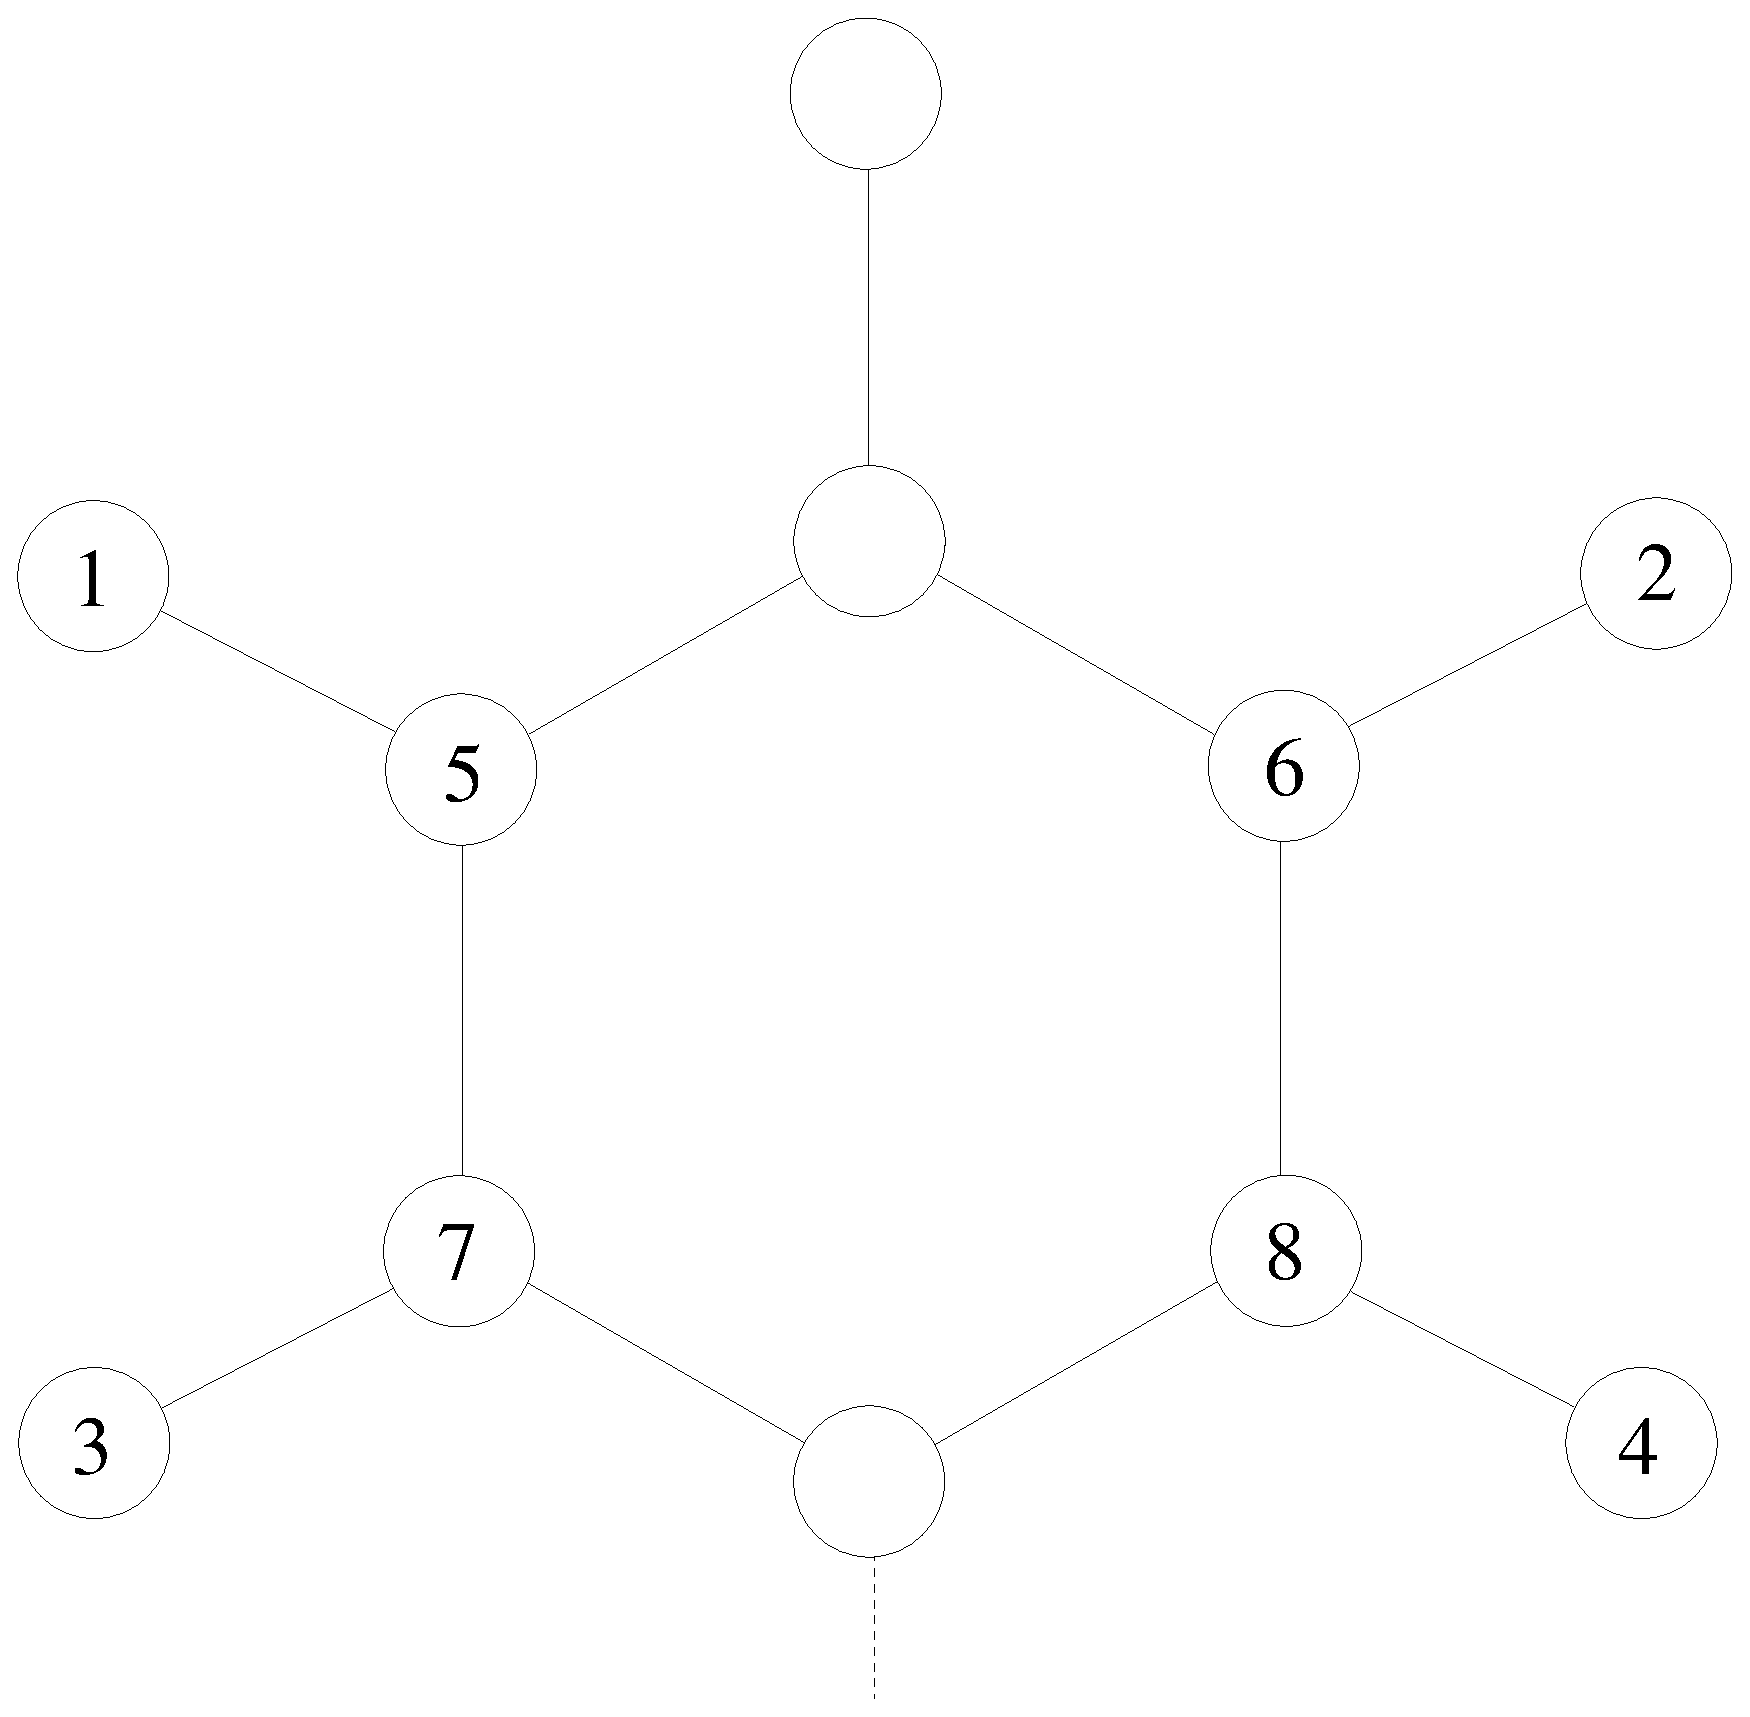
\includegraphics[width=0.5\textwidth]{PHE.eps}}
\end{figure}

For the phenylalanine example illustrated we must allow three other pairs of
atoms to exchange if we swap 7 and 8. Hence a suitable {\tt perm.allow} entry is
{\obeylines
1
2 3
7 8 5 6 1 2 3 4
}
Here $n=2$ and $s=3$: if we exchange 7 and 8 then we must also exchange 5 and 6,
1 and 2, and 3 and 4. There are two atoms in each of the three secondary sets, 
since we have specified 7 and 8 as the two primary atoms.

Here is an example {\tt perm.allow} file for a water trimer using
the flexible {\it QTIP4PF\/} potential, where the energy is invariant to permutations
of water molecules and to exchanges of hydrogens in the same molecule. However,
hydrogens cannot exchange between different oxygens:
{\obeylines
4
3 2
1 4 7 2 3 5 6 8 9
2 0 
2 3
2 0 
5 6
2 0 
8 9
}
The first group of three oxygens has two atoms that must move with each oxygen,
i.e.~atoms 2 and 3 for oxygen 1, etc. Hydrogen permutations for each oxygen are
allowed by the three following groups. This scheme allows atoms to appear in more 
than one group. There must be a group containing each complete set of permutations
in order for permutation-inversion isomers to be recognised. The format
is compatible with an older scheme, where only pair swaps were allowed for
associated atoms, but now allows for more general permutations.

Scripts to generate allowed permutations automatically for CHARMM and AMBER are available from
the group web site. It is essential to use symmetrised versions of the corresponding
force fields! 


\item {\it PLUS\/}: when combined with keywords {\it NEON\/} or {\it ARGON\/}
uses a diatomics-in-molecules potential for the singly charged cation.

\item {\it PMAX max\/}: {\it max\/} is the maximum probability of dihedral angle twisting for {\it AMBER\/}.

\item {\it PMIN min\/}: {\it min\/} is the minimum probability of dihedral angle twisting for {\it AMBER\/}.

\item {\it POWER ipow\/}: {\it ipow\/} is the initial power for shifts in the old line minimisation routine
for conjugate gradient. LBFGS minimisation should be used instead.

\item {\it PROJI\/}: turns on projection operator to enforce $I$ point group symmetry
in {\bf mylbfgs.f}. The geometry is projected after every proposed step.

\item {\it PROJIH\/}: turns on projection operator to enforce $I_h$ point group symmetry
in {\bf mylbfgs.f}. The geometry is projected after every proposed step.

\item {\it PTMC histmin histmax ptemin ptemax pttmin pttmax exchprob nequil ptsteps nenrper hbins\/}: 
requests a standard parallel tempering MC run.
This keyword also specifies the energy range for the histogram of quench energies,
{\it histmin\/} to {\it histmax\/},
the energy range for the histogram of instantaneous configurations, {\it ptemin} to {\it ptemax}, 
the temperature range ({\it pttmin} and {\it pttmax}), 
the probability of attempting an exchange {\it exchprob}, the 
number of equilibration steps, {\it nequil},
the number of parallel tempering MC steps without quenching,  {\it ptsteps},
the number of bins for the histogram of instantaneous potential energy, {\it nenrper}, and
the number of bins for the histogram of quench energies, {\it hbins}.
Should be used together with the {\it MPI\/} keyword. % and {\it BINSTRUCTURES\/} keywords.
(This option is only available if the source is compiled with an MPI enabled.)  

\item {\it PULL a1 a2 f\/}: apply a static force to the potential, equivalent to adding
the term $V_{\rm pull}=-f(z_{a1}-z_{a2})$. Here $z_{a1}$ and $z_{a2}$ are the $z$
coordinates for atoms $a1$ and $a2$, and $f$ specifies the force.
This potential is designed to simulate a pulling experiment with static force where
a molecule is pulled along the $z$ axis from atoms $a1$ and $a2$.

\item {\it QCUTOFF qcut\/}: {\it qcut\/} is a distance cut-off for Coulomb interactions in {\it AMBER\/}.

\item {\it QMAX cgmax\/}: {\it cgmax\/} is the tolerance for the 
RMS force in the final set of quenches that are used to produce
the output for file {\tt lowest}. The default is 
{\it cgmax\/}$=10^{-3}$, but the appropriate value depends upon the system in question.
{\it TIGHTCONV} can be used instead.

\item {\it QUAD\/}: requires documentation.

\item {\it QUCENTRE\/}: sets the centre of coordinates to the origin (0,0,0) before each MC step is taken (so after each quench), but not during the minimisation itself unlike {\it CENTRE}. 

\item {\it RADIUS radius\/}: sets the radius of the container that prevents particles
evaporating during quenches. If unset the program calculates an appropriate value
based upon the volume per particle for close-packed material and the known pair
equilibrium distance for the given potential. The formula employed is
$$  RADIUS=r_e\left[1 + \left(3 n \over 4\pi\sqrt{2}\right)^{1/3}\right], $$
where $n$ is the number of atoms and $r_e$ is the pair equilibrium
separation.\cite{kittel76} The `1' in this formula is to allow some extra space for
more open structures.

\item {\it RANDOMSEED\/}: specifies that the random number generator should be seeded with system time after each quench, allowing simple parallel use. Currently functional only for the CHARMM and AMBER potentials.

\item {\it RANSEED i\/}: integer seed for the random number generator.

\item {\it RCUTOFF rcut\/}: {\it rcut\/} is a distance cut-off in {\it AMBER\/}.

\item {\it RESIZE resize\/}: all the coordinates are multiplied by {\it resize\/} after
they have been read in, before any other operations are performed. This command is useful
for scaling results obtained with one potential for a system with a different pair
equilibrium distance.

\item {\it RESTART\/ nrelax nhs\/}: reseed runs if a step in not accepted
within twice {\it nrelax} steps.
{\it nhs} is the number of hard sphere moves used to produce the new starting configuration.
If {\it nhs=0} (the default) then the geometry is changed by reseeding.

\item {\it RESTORE\/ dumpfile intEdumpfile\/}: restore a previous {\tt GMIN} run from a {\it dumpfile}.
The number of basin-hopping steps performed will be the difference between the number
requested for the run that produced the dumpfile, minus the number that were completed
at the point the dumpfile was created. This option is not available before version 2.3.
If you are using the {\it A9INTE\/} keyword, you can specify the interaction enthalpy
dump file to restore from as a second arguement.

\item {\it RGCL2\/}: specifies a DIM rare gas-Cl$_2$ potential.

\item {\it RINGROTSCALE factor\/}: when applying cartesian moves with CHARMM, amino acid rings are moved as rigid units. Setting {\it factor} (default 0.0) between 0.0 and 1.0 will apply a random rotation to these rings during step taking. The suggested value is 0.1 to prevent the regular formation of high energy structures. 

\item {\it RKMIN\/}: specifies a Runga-Kutta minimisation scheme. 
Very inefficient.

\item{\it RMS rmslimit rmstol rmssave lca best}: used with {\it CHARMM} keyword to
specify that the RMSD compared to a reference geometry is calculated. The reference geometry must 
be given in xyz-format in an additional file {\tt compare}. {\it rmssave} is an integer 
that specifies the number of lowest energy geometries and RMSD $\le$ {\it rmslimit}
to save. Geometries are only saved if their RMSD's are more than {\it rmstol} 
different. The flag {\it lca} controls whether the all-atom RMSD ({\it lca}=0) or the $C_{\alpha}$-RMSD 
({\it lca}=1) is calculated. The flag {\it best} determines which structure is compared to the reference
after each quench. {\it best}=0 implies the current quench minimum and {\it best}=1 implies the current best (lowest energy) minimum. If {\it TRACKDATA} is also specified, the RMSD calculated after each quench is produced in the file `rmsd' in gnuplot readable format.

\item {\it ROTAMER maxchange pselect occuw (centre cutoff)\/}: Used with AMBER9 only. Specifies that rotamer moves should be taken. Every step, up to {\it maxchange} rotamers may be selected with a probability {\it pselect}. {\it occuw} determines the minimum \% occupation a rotamer must have to be selected from the library\cite{lovelljm00} when making a change. For example, {\it occuw} $= 0.004$ restricts possible rotamer choice to those with a greater than 0.4\% occupation. If you want to focus rotamer changes around a ligand/binding pocket, the optional {\it centre} and {\it cutoff} arguements may be used. {\it centre} specifies the residue of interest (for example a ligand), and {\it cutoff} the limiting distance from this centre that rotamers may be changed. The selection probability decreases linearlly from the {\it centre} residue. To use these moves, you need three files found in the SCRIPTS directory: PdbRotamerSearch, penultimate.lib and rotamermove.csh in your working directory for each run. 

\item {\it SAVE nsave\/}: {\it nsave\/} is an integer that specifies the number of lowest
energy geometries to save and summarise in the file {\tt lowest}. 
Arrays are now dynamically allocated, so any positive integer can be specified.

\item {\it SAVEINTE nsaveinte\/}: {\it nsaveinte\/} is an integer that specifies the number of lowest
interaction enthalpy geometries to save and summarise in the file {\tt intelowest}. See {\it A9INTE\/}. 

\item {\it SETCENTRE x y z\/}: Sets the centre of mass/coordinates (before the initial quench) to ({\it x,y,z\/}). For example, {\it SETCENTRE 0.0 0.0 0.0\/}
would translate the centre of mass to the origin.

\item {\it SC nn mm sig sceps scc\/}: specifies a Sutton-Chen potential\cite{suttonc90} with
parameters $n=${\it nn\/}, $m=${\it mm\/}, $a$={\it sig\/}, $\epsilon=${\it sceps\/} and 
$c=${\it scc\/}.

\item {\it SEED nsstop\/}: if the {\it SEED\/} keyword appears then the program
looks for a file {\tt seed} containing coordinates, which are used to `seed' the new run.
The number of coordinates given in this file should be no more than one less than the number
given in {\tt coords}. The specified coordinates are frozen from the first step until 
step {\it nsstop\/}.

\item {\it SHIFTCUT\/}: specifies a shifted-truncated potential for bulk binary Lennard-Jones.

\item {\it SIDESTEP smax\/}: specifies the maximum step in Cartesian coordinates for side-chains
in {\it AMBER\/}.

\item {\it SLOPPYCONV bgmax\/}: specifies a basin-hopping run (as opposed to standard MC
on the untransformed surface). {\it bgmax\/} is the convergence criterion
for the RMS force in the basin-hopping
quenches. If this criterion is too strict then the run time will be greatly increased.
If it is too sloppy then the performance of the algorithm is impaired. Different values
are needed for different potentials. {\it BASIN} can be used instead.

\item {\it SORT}: for pairwise potentials the atoms can be sorted from most to least
strongly bound. The {\it SORT} keyword enables this sorting for the coordinates printed
in file {\tt lowest}. This can be useful for seeding subsequent runs by removing the
most weakly bound atoms. This sort is not set by default and is meaningless if the
pair energies are not computed.

\item {\it STAR}: specifies an excited state calculation for Ar$^*_n$ or Ne$^*_n$ for
a diatomics-in-molecules potential when used with {\it NEON\/} or {\it ARGON\/}.

\item {\it STEP step astep ostep block\/}: specifies the maximum step sizes. {\it step\/} is
for the maximum change of any Cartesian coordinate and {\it astep\/} specifies a tolerance
on the binding energy of individual atoms (if available, i.e.~for Morse and LJ) below
which an angular step is taken for that atom. See the following section for more details.
{\it ostep\/} is the maximum displacement of an axis-angle coordinate for a rigid body system
and {\it block\/} (an integer) is the block size for which separate translational and orientational
displacements will be made for rigid bodies. Omitting {\it block\/} or using a value of zero results in
translational and orientational steps being taken simultaneously
for rigid bodies. The default values for {\it step\/},
{\it astep\/} and {\it ostep\/} are all 0.3 and the default value of {\it nblock\/} is zero.

\item {\it STEEREDMIN smink sminkinc smindiststart smindistfinish sminatoma sminatomb\/}: specified steered 
minimisation should be performed (must be used with {\it AMBER9}). For a protein/ligand system, this adds a translation
to the MC move. The vector between the centre of coordinates of groups A and B (as defined in the file movableatoms)
is calculated and set to {\it smindiststart}. During the following minimisation, a restoring force is applied to 
the ligand. The harmonic force constant is initially zero, and rises by {\it sminkinc} every LBFGS step up to a
maximum of {\it smink}. The force is applied until the A->B distance is less than {\it smindistfinish}.  

\item {\it STEPS mcsteps tfac\/}: determines the length of the
basin-hopping run through the integer {\it mcsteps\/} and the annealing protocol through
the real variable {\it tfac\/}. The temperature is multiplied by {\it tfac\/}
after every step in each run. 

\item {\it STICKY nrbsites, sigma\/}: specifies a `sticky patch' potential with {\it nrbsites}
sites in the rigid body reference and a value of {\it sigma} for the $\sigma$ parameter.

\item {\it STOCK mu lambda}: specifies a Stockmeyer potential with parameters
$\mu$ and $\lambda$, respectively.

\item {\it STRAND}: specifies a system of $\beta$ strands coded using the rigid body formalism.

\item {\it SW\/}: specifies the Stillinger-Weber Si potential.

\item {\it SYMMETRISE int tol1 tol2 tol3 tol4 tol5 qmax mdiff d}: specifies that the symmetrisation
routine should be called every {\it int} steps. The five {\it tol} parameters are tolerances
for various parts of the routine: 
{\it tol1} is used in {\bf ptgrp.f} in defining orbits; 
{\it tol2} is the distance tolerance used in {\bf ptgrp.f} to define point group symmetry operations;
{\it tol3} is the maximum relative difference in principal moments of inertia used to
diagnose point groups with degenerate irreducible representations in {\bf ptgrp.f};
{\it tol4} is the distance cutoff used to determine if a symmetry element has been lost in {\bf symmetry.f}.
Since we are dealing with approximate symmetries, this parameter may be larger than {\it tol2}.
It is compared to the largest atomic displacement divided by the corresponding radius
for the closest permutation.
{\it tol4} is also used to test whether atoms lie on a given symmetry element, and in testing 
whether orbits generated from `floaters' are actually contained in the core.
{\it tol5} is generally to check for atom clashes in {\bf symmetry.f}, including analysis of
missing sites in orbits, as well as overlap between orbits generated from `floaters' and
previous core or new orbit sites.
{\it qmax} is the maximum number of quenches allowed for each call to {\bf symmetry.f}.
{\it mdiff} is used to test whether a generated symmetry operation is new. If any of the nine
components of the corresponding $3\times3$ matrix differs by more than {\it mdiff} from an
existing matrix then the operations are considered to be different.
{\it d} is the exponential factor used in constructing a centre of mass that is biased towards
core atoms. The contribution of each atom is weighted by $\exp(-dx(i))$, where $x$ is the 
centre of mass distance of atom $i$ on the previous cycle.

\item {\it TABOO nlist\/}: specifies a taboo list of the {\it nlist\/} lowest minima should be maintained.

\item {\it TARGET target1 target2 $\cdots$\/}: specifies any number of target energies. 
The current run stops in an orderly
fashion if the current quench energy is within {\it econv\/} of any target (see {\it EDIFF\/}).

\item {\it TEMPERATURE temp\/}: defines the temperature, {\it temp\/}, at which the 
MC runs are conducted. Different values can be specified for serial `parallel' runs if
{\it PARALLEL} is set.
For true parallel basin-hopping use the {\it BHPT\/} keyword and omit {\it TEMPERATURE\/}.

\item {\it TETHER hdistconstraint hwindows ExtrapolationPercent lnHarmFreq}: requests a calculation of the vibrational density of
states for a given minimum. {\it hdistconstraint} is the minimised average radius of the basin of attraction to which the minimum
belongs, {\it hwindows} is the number of potential energy windows into which a WL simulation is split. {\it 
ExtrapolationPercent} is the percentage of the whole potential energy spectrum, for which the density of states is estimated from
the harmonic approximation and not sampled. {\it lnHarmFreq} the log product of positive Hessian
eigenvalues.

\item{\it THOMSON q\/}: specify the Thomson problem for unit charges on a sphere.
If {\it q\/} is present it is taken to be the charge on one particle, which can
therefore be different from all the other unit charges and is read as a real number.

% Doesn't appear to be coded?
% \item {\it THRESHOLD \/}: specifies threshold acceptance of steps. The change in potential energy must be
% less than the value of the {\it TEMPERATURE\/} variable for a step to be accepted.

\item {\it TIGHTCONV cgmax\/}: cgmax is the tolerance for the
RMS force in the final set of quenches that are used to produce
the output for file {\tt lowest}. The default is
{\it cgmax\/}$=10^{-3}$, but the appropriate values depend upon the system in question.
{\it QMAX} can be used instead.

\item {\it TIP n\/}: specifies a TIP{\it n\/}P intermolecular potential for rigid body water molecules.
$\ \le n \le 5$.

\item {\it TOLBRENT tolb\/}: parameter for {\it DBRENT\/} minimisation. 
Inefficient compared to LBFGS.

\item{\it TOMEGA}: used with the {\it CHARMM} keyword to specify that peptide bonds will be twisted along with all other dihedrals.

% \item {\it TN\/}: specifies a truncated Newton minimisation scheme. 
% Inefficient compared to LBFGS.

\item {\it TOSI app amm apm rho\/}: specifies the Tosi-Fumi potential\cite{tosif64}
with parameters $A_{++}$, $A_{--}$, $A_{+-}$ and $\rho$.

\item {\it TRACKDATA}: produces `energy.dat' and `markov.dat' containing the quench number and 
associated energy and markov energy in two columns and `best.dat', containing the current quench number and the current lowest
total energy. If {\it RMS\/} is also specified, a file called `rmsd.dat' is produced containing the RMSD from a reference structure.
See {\it RMS\/} for more information. This allows plotting with gnuplot to monitor convergence of multiple runs.
If {\it A9INTE} is also specified, two additional output files are produced, `intE.dat' containing the quench number and associated interaction
enthalpy, and `bestintE.dat' containing the quench number and current lowest interaction enthalpy. This keyword does not yet function for MPI runs.

\item {\it TSALLIS q\/}: specifies that steps are accepted/rejected using Tsallis statistics with the
given value of {\it q\/}, rather than the usual Boltzmann condition.

\item {\it TWOPLUS\/}: when combined with keywords {\it NEON\/} or {\it ARGON\/}
uses a diatomics-in-molecules potential for the doubly charged cation.

\item {\it UACHIRAL\/}: MUST be included when using ff03ua, the AMBER united atom forcefield unless you have disabled the checks for inverted chiral carbons
 with {\it NOCHIRALCHECKS\/}. {\it UACHIRAL\/} ensures the correct impropers are used to define sidechain chirality when HB hydrogen is missing. 

\item {\it UPDATES nup\/}: {\it UPDATES\/} is the number of previous steps saved in the LBFGS routine,
default 4.

\item {\it VGW ljsigma ljepsilon taumaxsg taumaxfg}: Specifies use of VGW quantum quenching in place of
classical minimization routines such as LBFGS. {\it ljsigma} and {\it ljepsilon} are the corresponding Lennard-Jones
parameters that must be specified, and taumaxsg and taumaxfg are the maximum value of ``imaginary'' time $\tau$ (inverse tempertaure) for the propagation.
The former pertains to the faster ``single-particle'' SP-VGW used for quenching during the MC runs, and the latter for the more accurate
``fully-coupled'' VGW used for the final quenching (analogous to the tight convergence of the LBFGS). A $\tau$ of at least
2.5 is recommended for the SP-VGW and 5.0 for the FC-VGW. A file {\it vgwdata} containing the masses (in a.m.u.) of all particles, in order of the location
of their {\it xyz} coordinates in ``{\it coords}'' must be present (e.g. for a 38 atom Ne cluster, {\it vgwdata} will have 38 lines of ``{\it 20}''). Different
masses are permitted, though the current version allows for only one set of LJ parameters. 

\item{\it VGWCPS on magnitude}: Specifies use of contraining potential for SP-VGW (sloppy convergence), as clusters expand during quantum quenching
with decreasing mass. 1 or 0 for {\it on} corresponds to on/off,
and magnitude should range from 1 to 1000, with 1 having minimal effect, 1000 being highly constrained. Default value is ``on'', with magnitude 1.

\item{\it VGWCPF on magnitude}: Same as VGWCPS but for FC-VGW, used for the final, full quenching (tight convergence).

\item{\it VGWTOL magnitude}: Absolute tolerance parameter for differential equation solver used for VGW quenching. Default value is 0.0001.
For highly quantum or ``stiff'' systems this may need to be increased, while it may be decreased for ``softer'' or less quantum systems to enhance
speed.
 
\item {\it VISITPROP}: if specified the Wang-Landau convergence is governed by proportionality of visits to the current value of
the modification factor, and not the histogram flatness criterion \cite{ZhouB03}.

\item {\it WELCH $A_{++}\ A_{--}\ A_{+-}\ \rho\ Q_+\ Q_-\ \alpha_+\ \alpha_-$\/}: specifies a Welch binary
salt potential with the parameters indicated.

\item {\it ZETT1\/} and {\it ZETT2\/}: specify the Zetterling potentials.
% </kwd>
\end{itemize}

\section{Angular Steps}

For pure pair potentials the total energy can be broken down into a sum of binding
energies for the individual atoms. This is coded for the Morse and LJ potentials.
If the binding energy of any atom is lower than that of the most tightly bound atom
multiplied by the variable {\it astep\/} (see the {\it STEP\/} command above) then
that atom is randomly replaced on the sphere of radius equal to that of the atom furthest
from the centre of mass. Hence if {\it astep\/} is zero angular steps will never be taken,
and the closer this parameter is to one the more atoms will undergo such displacements.
If the step sizes are adjusted to give the required acceptance ratio then both {\it step\/} and
{\it astep\/} are multiplied or divided by $1.05$ every {\it naccept\/} steps depending
upon the current acceptance ratio. If {\it FIXSTEP\/} has been specified then the temperature
is adjusted in the same way and {\it step\/} and {\it astep\/} are unchanged.

% <systems>
\section{Some Recognised Systems}

\subsection{AMBER}

Specifies the AMBER force field. Coordinates are read from file {\tt coords.amber}.
See also associated keywords {\it PMAX\/}, {\it PMIN\/}, {\it NMAX\/}, {\it NMIN\/},
{\it SIDESTEP\/}, {\it RCUTOFF\/}, {\it QCUTOFF\/} and {\it FAKEWATER\/}.

\subsection{Binary Lennard-Jones}

If the {\it BINARY\/} keyword is specified then a binary Lennard-Jones
potential is used\cite{sastryds98}. {\it PERIODIC\/} must also be
specified. Reduced units are used with $\epsilon_{\rm AA}=\sigma_{AA}=1$.
{\it BLJCLUSTER\/} specifies a binary Lennard-Jones cluster.

\subsection{BLN Off-Lattice Protein Model}
\label{sec:BLN}

The general three-colour bead protein model is specified by keyword {\it BLN}.
The potential follows the form described in
{\it Proc.~Natl.~Acad.~Sci.~USA}, {\bf 100}, 10712, 2003, expect that
the coefficients $A_i$, $B_i$, $C_i$ and $D_i$ include a factor of $\epsilon$
explicitly.

{\arraycolsep0pt\begin{eqnarray}
V&\,=\,&\frac{1}{2} K_r\sum_{i=1}^{N-1}(R_{i,i+1}-R_{\rm e})^2
 +\frac{1}{2} K_\theta\sum_i^{N-2}(\theta_i-\theta_{\rm e})^2 \nonumber\\
 &&+\,\epsilon\sum_i^{N-3}\Big[A_i(1+\cos\varphi_i)+B_i(1-\cos\varphi_i) \nonumber\\
  && \qquad +C_i(1+\cos3\varphi_i)+D_i\left(1+\cos\left[\varphi_i+\pi/4\right]\right)\Big] \nonumber\\
 &&+\,4\epsilon\sum_{i=1}^{N-2}\sum_{j=i+2}^N \left[S_{12}\left(\frac{\sigma}{R_{ij}}\right)^{\!12}
    +S_6\!\left(\frac{\sigma}{R_{ij}}\right)^{\!6}\right],
\label{barrelpot}
\end{eqnarray}}
\noindent where $R_{ij}$ is the separation between beads $i$ and $j$ and
the units of distance and energy are $\sigma$ and $\epsilon$, respectively.
The first term represents the bonds linking successive beads in the linear chain, and a 
value of $K_r=231.2\,\epsilon\sigma^{-2}$ was used in most of the work on the 
Honeycutt and Thirumalai frustrated 46-bead model.
The second term is a sum over the bond angles, $\theta_i$, defined by the triplets
of atomic positions ${\bf R}_i$ to ${\bf R}_{i+2}$, and values
$K_\theta=20\,\epsilon\,{\rm rad}^{-2}$ and $\theta_{\rm e}=105^\circ$ were
used for the 46-bead model.
The third term
is a sum over the dihedral angles, $\varphi_i$, defined by the quartets ${\bf R}_i$ to
${\bf R}_{i+3}$. 
In the 46-bead model $A_i=C_i=1.2$ if the quartet involved no more than one N monomer, generating
a preference for the {\it trans\/} conformation ($\varphi_i=180^\circ$), whereas if two or three
N monomers are involved then $A_i=0$ and $C_i=0.2$.
This choice makes the three neutral
segments of the chain flexible and enables them to accommodate turns.
A general specification of these parameters is possible in the new BLN framework
via the auxiliary file {\tt BLNsequence}.
The last term in (\ref{barrelpot}) represents the nonbonded interactions.
In the current BLN implementation $R_{\rm e}$ is set equal to $\sigma$, i.e.~to 
unity in reduced units.

An appropriate {\tt BLNsequence} file for the usual 46-bead model contains the following
lines:

{\obeylines
\noindent comment: $S_{12}>0$ and $S_6<0$ for B-B, L-L and L-B, N-L and N-B and N-N
\noindent 1.0D0 -1.0D0
\noindent 0.33333333333333D0 0.33333333333333D0
\noindent 1.0D0 0.0D0
\noindent comment: coefficients A, B, C, D
\noindent comment: for Helical, Extended and Turn residues in order, four per line
\noindent 0.0D0 1.2D0 1.2D0 1.2D0
\noindent 0.9D0 0.0D0 1.2D0 0.0D0
\noindent 0.0D0 0.0D0 0.2D0 0.0D0
\noindent LBLBLBLBBNNNBBBLBLBBBNNNLLBLLBBLLBNBLBLBLBLNNNLBBLBLBBBL
\noindent EEEEEETEHTHEEEEEEEEHHEHHHHHHHHHHEHTEEEEEEETTTEEEEEEEE
}

\noindent The penultimate line defines the sequence, and the final line
defines which set of $A_i$, $B_i$, $C_i$ and $D_i$ parameters apply to which 
parts of the structure.\cite{BrownFH03}


\subsection{Diatomics-in-Molecules}

At present diatomics-in-molecules (DIM) potentials are available for various
clusters, which are specified by the line {\it ARGON\/}, {\it NEON\/},
{\it ARNO} or {\it RGCL2\/} in {\tt data}.
Further keywords specify the precise nature of the system for argon or
neon clusters: {\it NEUTRAL\/} for ground state neutral
clusters, {\it PLUS\/} for a single positive charge, {\it TWOPLUS\/} for a double positive
charge, {\it STAR\/} for an electronic excited state and {\it DIPOLES\/} for the first order
induction energy in a charged system. Rare gas-Cl$_2$ and Ar$_N$-NO DIM potentials
are specified by the {\it RGCL2\/} keyword.

\subsection{DFT-based tight-binding}

If the {\it DFTB\/} keyword is specified then a DFT-based tight-binding potential
is used. See also the {\it MULTIPLICITY\/} keyword.

\subsection{LB2}

This keyword specifies the potential\cite{LB299a,LB299b,LB204}
\begin{equation}
V = \frac{\epsilon}{2} \sum_{i<j} \left[ \left(\frac{r_{ij}}{\sigma}\right)^2+
\left(\frac{\sigma}{r_{ij}}\right)^2\right],
\end{equation}
where $\epsilon$ and $\sigma$ are set to unity.

\subsection{Farkas}

The Farkas potentials for aluminium and nickel are specified by keywords {\it FAL\/} and
{\it FNI\/}, respectively.

\subsection{Lennard-Jones}

This is the default potential if nothing is specified in {\tt data}. Reduced units are
assumed with $\epsilon=\sigma=1$.

\subsection{Morse}

This potential is specified by the line {\it MORSE rho\/} in {\tt data} and gives a
a Morse potential with $D=r_e=1$. 
The remaining range parameter,\cite{braierbw90,doyewb95,doyew96a} $\rho$, has a default 
value of six.

\subsection{P46}

Keyword {\it P46\/} specifies a 46-bead three-colour model polypeptide. 
See also the more general implementation of the BLN model in \S \ref{sec:BLN}.

\subsection{Stillinger-Weber Si}

Specified by the keyword {\it SW\/}.

\subsection{Sutton-Chen}

These potentials\cite{suttonc90} are specified by the line {\it SC nn mm sig sceps scc\/} in {\tt data},
as described above. 

\subsection{Tight-binding}

Tight-binding potentials for silicon are specified by the keywords {\it MSORIG\/} 
and {\it FRAUSI\/}.
These potentials also understand the 
keywords {\it PERIODIC\/} and {\it CUTOFF\/} which enable calculations on bulk material
to be performed and a cutoff to be imposed on either cluster or bulk calculations.
Keyword {\it ANGSTROM\/} specifies coordinates in \AA ngstrom rather than bohr.

\subsection{TIP{\it n\/}P Water}

The TIP{\it n\/}P intermolecular water potentials are specified by the keyword {\it TIP\/}.
{\it n\/}=1 through 5 are currently coded. For $N$ water molecules the first $N$ lines of
the {\tt coords} file are the coordinates of a reference origin in each of $N$ rigid molecules,
and the next $N$ lines are angle-axis coordinates. The same convention is used in the output
file {\tt lowest}. The lowest minima are also dumped in xyz format in the file {\tt tip.xyz}.

\subsection{Tosi-Fumi}
 
Keyword {\it TOSI\/} specifies a Born-Mayer potential of the form
$$ E = \sum_{i<j}\left[ {q_i q_j\over r_{ij}} + A_{ij}\exp(-r_{ij}/\rho) \right]. $$
The sum runs over all ions. Tosi-Fumi\cite{tosif64} parameters in atomic units should be
entered after the Tosi keyword in the order $A_{++}$, $A_{--}$, $A_{+-}$, $\rho$.
The ions are specified in file {\tt coords} using PL and MI for plus and minus, respectively,
and can be in any order. There need not be equal numbers of positive and negative ions.
Note that the Welch potential has been fitted to include ion polarizabilities and is described below.

\subsection{Welch}This keyword specifies a Welch potential\cite{welchld76,phillipscb91} of the form
\begin{eqnarray*}
% I have tried \bm \boldsymbol etc. but I can't get a bold mu?!
E &= \sum_{i<j}\Bigg[ {\D q_i q_j\over\D  r_{ij}} + A_{ij}\exp(-r_{ij}^{\rm eff}/\rho)
              -{\D q_i({\boldsymbol \mu}_j\cdot{\bf r}_{ij})\over\D  r_{ij}^3}
              -{\D q_j({\boldsymbol \mu}_i\cdot{\bf r}_{ji})\over\D  r_{ij}^3} \\
             &-3{\D   ({\boldsymbol \mu}_i\cdot{\bf r}_{ij})
                   ({\boldsymbol \mu}_j\cdot{\bf r}_{ij})\over\D  r_{ij}^5}
              +{\D  {\boldsymbol \mu}_i\cdot{{\bf{\mu}}}_j\over\D  r_{ij}^3}\Bigg]
              +\sum_i {\D \mu_i^2\over\D 2\alpha_i}, \\
\end{eqnarray*}
where
$$ {\bf r}_{ij}^{\rm eff}={\bf r}_{ij}+{{\boldsymbol \mu}_i\over Q_i}-{{\boldsymbol \mu}_j\over Q_j},
    \qquad r_{ij}^{\rm eff}=\left|{\bf r}_{ij}^{\rm eff}\right|. $$
Welch parameters in atomic units should be
entered after the Welch keyword in the order $A_{++}$, $A_{--}$, $A_{+-}$, $\rho$, $Q_+$,
$Q_-$, $\alpha_+$, $\alpha_-$.
The ions are specified in {\tt coords}  using atom types PL and MI for plus and minus, respectively,
and can be in any order. There need not be equal numbers of positive and negative ions.

% </systems>

% <examples>

\section{Example {\tt data} Files}

A basin-hopping run of 10,000 MC steps at reduced temperature $0.8$ for the Lennard-Jones potential
with a constant temperature specified by the `1.0' on the {\it STEPS\/} line.
Seeding occurs for the first 100 steps, so a file {\tt seed} is required in the 
working directory. The final quenches to produce the output in {\tt lowest} are much
tighter than the relatively `sloppy' quenches for the basin-hopping run (compare the
{\it SLOPPYCONV\/} line with the {\it TIGHTCONV\/} line). The maximum number of iterations per
conjugate gradient step is 250 for the sloppy quenches and 500 for the tight quenches.
The initial linear and angular step parameters are 0.36 and 0.4, and these are adjusted
every 50 steps to try and achieve an acceptance ratio of 0.5.

\medskip
\begin{tabular}{ll}
SLOPPYCONV & 0.01 \\
TIGHTCONV & 1.0D-3 \\
SORT \\
MAXIT & 250 500 \\
STEPS & 10000 1.0 \\
STEP & 0.36 0.4 \\
TEMPERATURE & 0.8 \\
\end{tabular}
\medskip

\noindent The next example is similar to the above but employs parameters that seem
to be suitable for a Morse potential with $\rho=6$.

\medskip
\begin{tabular}{ll}
SLOPPYCONV & 0.01 \\
TIGHTCONV & 1.0D-3 \\
SORT \\
EDIFF & 0.01\\
MORSE & 6.0\\
MAXIT & 200 500\\
STEPS & 10000 1.0\\
STEP & 0.35 0.4\\
TEMPERATURE & 0.6\\
\end{tabular}
\medskip

\noindent Global optimisation for a water cluster using the TIP4P potential.
The initial step sizes for translational and orientational rigid-body coordinates are
0.6 and 0.9, respectively, and the block size for separate translational and orientational
steps is 200.

\medskip
\begin{tabular}{ll}
SLOPPYCONV & 0.01 \\
TIGHTCONV & 0.0001 \\
TIP & 4 \\
CENTRE & \\
MAXIT & 1000 1000\\
STEPS & 50000 1.0\\
STEP & 0.6 0.0 0.9 200 \\
TEMPERATURE & 5.0\\
\end{tabular}
\medskip

\noindent The following input file specifies a basin-sampling run to calculate the density of states for 
a LJ$_{13}$ cluster. The system is
confined to a spherical container of radius $1.8\,\sigma$, 
the geometry will be perturbed by $0.2\,\sigma$ at each step with no
angular steps allowed. The run will terminate after $1000000$ 
MC steps or when the WL convergence criterion {\it targetwl}
is satisfied, whichever is the earliest. Setting the temperature to zero indicates that 
a Wang-Landau type MC is used instead of
a conventional temperature-dependent MC run. In keyword {\it HISTOGRAM\/}
the energy of the global minimum of LJ$_{13}$ $-44.3268\,\epsilon$ is chosen
as the energy of the lowest bin {\it histmin}, the energy spectrum above that point is 
separated into $50$ bins of width $0.25$ each. The
starting modification factor and target number of WL iterations are 
{\it histfac} =$ 1.01$ and {\it targetwl} =$ 10$. A square root function
will  be used for decreasing the modification factor upon completion of each WL iteration, 
and the convergence schedule is regulated by {\it VISITPROP}.  


\medskip
\begin{tabular}{ll}
SLOPPYCONV & 0.001 \\
TIGHTCONV & 1.0D-3 \\
MAXBFGS &  0.1 \\
EDIFF & 0.003 \\
RADIUS &  1.8 \\
MAXIT & 1000 500 \\
STEPS & 1000000 1.0 \\
STEP  & 0.2 0.0 \\
TEMPERATURE & 0.0 \\
HISTOGRAM & -44.3268014195 $\:$ 0.2 $\:$ 1.1D0 $\:$ 50 $\:$ 0.5 $\:$ 10 $\:$ 0.2 \\
EQUILIBRATION 1 100 \\
FIXBOTH \\
BINSTRUCTURES 1 \\
VISITPROP \\
\end{tabular}
\medskip

% </examples>
% <end>
\section{Summary of Major Changes}

\subsection{12/10/10}
Changed to a more flexible scheme for atoms that must move together when
{\it PERMDIST\/} is pecified, in line with OPTIM and PATHSAMPLE.

\subsection{2/11/07}
Implementation of minimum image convention in distance minimisation.
{\it PERMDIST} keyword now made consistent with OPTIM and PATHSAMPLE
using {\tt perm.allow} file.

\subsection{31/12/06}
GMIN.2.3 introduced with MPI support by Tetyana Bogdan and David Wales.
New parallel tempering basin-sampling and
parallel tempering basin-hopping algorithms implemented.

\subsection{18/2/05}
\begin{itemize}
\item GMIN.2.0 recoded in fortran90 by Tetyana Bogdan and DJW. All arrays are now dynamically allocated.
\item Basin-sampling procedure programmed by DJW and developed by Tetyana Bogdan. See the new
{\it HISTOGRAM} keyword.
\item Interface to CHARMM added by David Evans and DJW. See keyword {\it CHARMM} and its associated 
parameters. Internal coordinate minimisation (written by David Evans and developed by Joanne Carr) 
is specified by keyword {\it INTMIN}.
\item Exploitation of approximate symmetry introduced through {\it SYMMETRY} keyword.
\item Bipartite matching implemented for matching closest permutational isomers
(thanks to Tomas Oppelstrup). Now used with 
the {\it PERMDIST} keyword, as well as the new taboo-type procedure introduced through keyword {\it AVOID}.
\item Cooperative moves introduced via keyword {\it COOPMOVE}.
\item Various new potentials have been added: {\it NATB} specifies a tight-binding potential
for sodium (can be guided by {\it GUPTA 21}); various Gupta potentials; Stockmeyer; sticky patches, etc.
\end{itemize}

\subsection{22/6/03}
\begin{itemize}
\item Support for rigid bodies added, e.g.~potentials {\it TIP\/}, {\it CAPSID\/} and {\it OTP\/}.
The centre-of-mass and angle-axis derivatives are calculated in subroutine {\tt rigidfunc.f}, so for pairwise
site-site potentials all that is needed are additional statement functions for these potentials and their
first derivative with respect to the distance.
\item Guiding potentials changed. The new keyword {\it GUIDE\/} allows specification of a parameter,
{\it guidecut\/}, the RMS force below which the real potential is used. 
\item Glue potential for lead added.
\item Keyword {\it TSALLIS\/} introduced for an alternative to the Metropolis
accept/reject step with Boltzmann statistics.
\item Keywords {\it BINARY\/}, {\it BLJCLUSTER\/} and {\it SHIFTCUT\/} introduced for binary LJ systems,
{\it ZETT1\/} and {\it ZETT2\/} for Zetterling potentials, {\it FAL\/} and {\it FNI\/} for Farkas Al and Ni
potentials, {\it ARNO\/}, {\it MULTIPLICITY\/} for {\it DFTB\/} and 
{\it AXTELL\/} for an additive Axilrod-Teller contribution.
Keywords {\it NEWJUMP\/} and {\it PNEWJUMP\/} for parallel runs with parallel tempering-like jumps
and {\it JUMPMOVE\/} for jump-walking parallel runs.
Keyword {\it TABOO\/} for runs with a taboo list.
\item Keyword {\it PERMDIST\/} added for runs that minimise the distance between two structures by permuting
atoms.

\end{itemize}

\subsection{15/10/99}
\begin{itemize}
\item Replaced conjugate gradient minimisation by the limited memory algorithm
      of Jorge Nocedal\cite{lbfgs}.
\item The convergence for {\it SLOPPYCONV\/} and {\it TIGHTCONV\/} is now
      based only on the RMS gradient. The energy change condition has gone.
\item New parameters for the LBFGS routine. {\it PRINTLEVEL\/} sets the 
      print level parameters, {\it UPDATES\/} the number of LBFGS updates
      before resetting and {\it GTOL\/} the tolerance for line minimisation.
\end{itemize}

\def\aciee{Angew.~Chem.~Int.~Ed.~Engl.}
\def\acp{Adv.~Chem.~Phys.}
\def\acr{Acc.~Chem.~Res.}
\def\ac{Acta.~Crystallogr.}
\def\ajp{Am.~J.~Phys.}
\def\am{Adv.~Mater.}
\def\apl{Appl.~Phys.~Lett.}
\def\ap{Ann.~Physik}
\def\Pa{Physica A}
\def\arpc{Ann.~Rev.~Phys.~Chem.}
\def\bbpc{Ber. Bunsenges. Phys. Chem.}
\def\bc{Biochemistry}
\def\cccc{Coll.~Czech.~Chem.~Comm.}
\def\cj{Comput.~J.}
\def\cpc{Comp.~Phys.~Comm.}
\def\cpl{Chem.~Phys.~Lett.}
\def\cp{Chem.~Phys.}
\def\crev{Chem.~Rev.}
\def\dalton{J.~Chem.~Soc., Dalton Trans.}
\def\el{Europhys.~Lett.}
\def\faraday{J.~Chem.~Soc., Faraday Trans.}
\def\fartrans{J.~Chem.~Soc., Faraday Trans.}
\def\fdisc{J.~Chem.~Soc., Faraday Discuss.}
\def\ic{Inorg.~Chem.}
\def\ijmpc{Int.~J.~Mod.~Phys.~C}
\def\ijqc{Int.~J.~Quant.~Chem.}
\def\jacers{J. Am. Ceram. Soc.}
\def\jacs{J.~Am.~Chem.~Soc.}
\def\jap{J.~Appl.~Phys.}
\def\jas{J.~Atmos.~Sci.}
\def\jcc{J.~Comp.~Chem.}
\def\jce{J.~Chem.~Ed.}
\def\jcis{J.~Colloid Interface Sci.}
\def\jcp{J.~Chem.~Phys.}
\def\jcscc{J.~Chem.~Soc., Chem.~Commun.}
\def\jcsft{J.~Chem.~Soc., Faraday Trans.}
\def\jetp{J.~Exp.~Theor.~Phys.~(Russia)}
\def\jmc{J.~Math.~Chem.}
\def\jmsp{J.~Mol.~Spec.}
\def\jmst{J.~Mol.~Structure}
\def\jncs{J.~Non-Cryst.~Solids}
\def\jpa{J.~Phys.~A}
\def\jphysc{J.~Phys.~C}
\def\jpca{J.~Phys.~Chem.~A}
\def\jpcb{J.~Phys.~Chem.~B}
\def\jpcm{J.~Phys.~Condensed Matter.}
\def\jpcssp{J.~Phys.~C: Solid State Phys.}
\def\jpcs{J.~Phys.~Chem.~Solids.}
\def\jpc{J.~Phys.~Chem.}
\def\jpfmp{J.~Phys.~F, Metal Phys.}
\def\jpsj{J.~Phys.~Soc.~Jpn.}
\def\jsp{J.~Stat.~Phys.}
\def\mg{Math.~Gazette}
\def\molphys{Mol.~Phys.}
\def\molp{Mol. Phys.}
\def\mrsb{Mater.~Res.~Soc.~Bull.}
\def\msr{Mater.~Sci.~Rep.}
\def\nat{Nature}
\def\njc{New J.~Chem.}
\def\pac{Pure.~Appl.~Chem.}
\def\phys{Physics}
\def\pla{Phys.~Lett.~A}
\def\phm{Philos. Mag.}
\def\pma{Philos.~Mag.~A}
\def\pmb{Philos.~Mag.~B}
\def\pml{Philos.~Mag.~Lett.}
\def\pnasu{Proc.~Natl.~Acad.~Sci.~USA}
\def\pnas{Proc.\ Natl.\ Acad.\ Sci.\  USA}
\def\pra{Phys.~Rev.~A}
\def\prbcm{Phys.~Rev.~B}
\def\prb{Phys.~Rev.~B}
\def\prc{Phys.~Rev.~C}
\def\prd{Phys.~Rev.~D}
\def\prep{Phys.~Reports}
\def\pre{Phys.~Rev.~E}
\def\prl{Phys.~Rev.~Lett.}
\def\prsa{Proc.~R.~Soc.~A}
\def\pr{Phys.~Rev.}
\def\psfg{Proteins: Struct., Func.~and Gen.}
\def\pssb{Phys.~State Solidi B}
\def\pss{Phys.~State Solidi}
\def\rmp{Rev.~Mod.~Phys.}
\def\rpp{Rep.~Prog.~Phys.}
\def\sci{Science}
\def\ss{Surf.~Sci.}
\def\tca{Theor.~Chim.~Acta}
\def\tetra{Tetrahedron}
\def\zfpd{Z.~Phys.~D}
\def\zpb{Z.~Phys.~B.}
\def\zpc{Z.~Phys.~Chem.}
\def\zpdamc{Z.~Phys.~D}
\def\zpd{Z.~Phys.~D}


\cleardoublepage
\phantomsection
\addcontentsline{toc}{chapter}{Bibliography}

\bibliographystyle{thesis}
\bibliography{GMINdoc}

\end{document}
% </end>
% </document>
